\pagestyle{fancy}
\fancyhead[R]{Física Nuclear y de Partículas: Tema 1}
\fancyhead[L]{4º Grado en Física}
\chapter{Partículas elementales: clasificación y propiedades}
Como introducción al estudio de la física de partículas (y a la física nuclear) vamos a estudiar el concepto de partícula fundamental y las propiedades de las mismas, permitiéndonos así clasificarlas.
\section{Introducción histórica y conceptual}
\subsection{La idea de simplicidad}
Según Anaxágoras (siglo V A.C) la materia estaba constituída por 4 elementos, a saber: Tierra, Aire, Fuego y Agua. Aunque como sabemos esta idea está muyy alejada de la realidad, nos introduce un concepto muy potente en la física: la \textbf{simplicidad}. \\\\
Toda teoría física busca explicar un fenómeno natural reduciéndolo a unos elementos mínimos, en nuestro caso las partículas fundamentales.\\\\
A lo largo de 24 siglos se fueron desglosando los 4 elementos de la naturaleza en otras partes más fundamentales y fue en 1869 cuando Mendeléyev clasificó los entonces conocidos 63 elementos ordenándolos según su masa atómica. Esta clasificación nos introducía mucha complejidad para entender la estructura de la materia pues pasábamos de 4 elementos a 63 pero era infinitamente más acertada que la clasificación de Anaxágoras.\\\\
A finales del siglo XIX se descubre el electrón y en la primera década del siglo XX se descubre el átomo (y el núcleo). No es hasta 1931 donde conseguimos ver los diferentes comoponentes del nucleo y recuperamos la simplicidad: sólo hacen falta 3 partículas ($e^-, p, n$) para describir toda la materia.\\\\ Este ambiente duraría poco pues con el descubrimiento de las antipartículas y de las partículas exóticas (muón, tau neutrinos...) recuperaríamos la complejidad alcanzando un número de $\sim 3000$ partículas conocidas. Aunque no está todo perdido pues el modelo estándar nos permite reducir a poco más de 15 las partículas fundamentales (conocidas).
\subsection{La escala}
La complejidad a la hora de describir la materia ha ido cambiando a medida que hemos podido ``ver'' elementos más \textbf{pequeños}, en la siguiente figura vemos cómo al hacer zoom a un átomo aumenta y disminuye su complejidad
\begin{figure}[h]
\centering
\begin{subfigure}[h]{0.3\textwidth}
    \centering
    \includegraphics[]{Diagramas Tema 1/Atomo.pdf}
    \subcaption{Átomo}
\end{subfigure}
\hfill
\begin{subfigure}[h]{0.3\textwidth}
    \centering
    \includegraphics[]{Diagramas Tema 1/NucleoAtomico.pdf}
    \subcaption{Núcleo atómico}
\end{subfigure}
\hfill
\begin{subfigure}[h]{0.3\textwidth}
    \centering
    \includegraphics[]{Diagramas Tema 1/ProtonEscala.pdf}
    \subcaption{Protón}
\end{subfigure}
    \caption{Diferentes escalas que nos encontramos en los principales sistemas de la física cuántica, cada una de las escalas tiene asociado un orden de energía.}
    \label{fig:T1 Escalas}
\end{figure}

Vamos a centrarnos en el átomo y el núcleo, como sabemos, los átomos están regidos por la interacción electromagnética, el potencial electromagnético es el Coulombiano, con lo que para distancias de $\unit[10^{-10}]{m}\equiv \unit[1]{\text{\AA}}$ 
\begin{equation*}
V\sim \frac{1}{r} \Rightarrow \expval{V}_\text{\AA} \sim\unit[10]{eV} \quad \text{para $d=\unit[1]{fm}$ tenemos} \quad \expval{V}_\text{fm} \sim\unit[1]{MeV}
\end{equation*}
Por lo tanto cuanto menor sea la distancia en la que queremos ver, mayor será la energía que necesitamos para ``ver''.\\\\
A medida que aumentamos la escala nos pueden aparecer nuevas interacciones, como es el caso de las interacciones débiles y fuertes ó las correcciones de estructura fina del átomo de hidrógeno como pueden ser la correción spin-órbita $\vec{L}\cdot \vec{S}$, el término de orden $p^4$ de la energía cinética y el término de Darwin; es éste último el que tiene mayor relevancia para nuestro ejemplo pues el núcleo atómico no es puntual, sino que es una distribución continua de carga, esto quiere decir que tendremos que estudiar la influencia de todos los puntos del núcleos sobre el electrón, es decir, es el desarrollo multipolar de las partículas que constituyen el átomo.
\subsection{Sistemas de partículas: Desintegraciones y estabilidad}
Hacia el año 2004 se conocían 111 elementos químicos aunque se habían sintetizado elementos de $Z=115$, poco a poco esos elementos se han ido caracterizando hasta alcanzar en 2021 el 118 \footnote{Se han sintetizado elementos más pesados pero aún no se han caracterizado}. Lo que nos permite apuntar que a pesar de que se encuentran nuevos elementos, la teoría sigue siendo válida.
\subsubsection{Estabilidad e inestabilidad de los núcleos}
El último núcleo estable que se conoce es el plomo-208, que contiene 82 protones y 126 neutrones. Por lo tanto todos los núcleos con mayor masa tenderán a decaer en este núcleo (o similar).\newpage
En los elementos de $Z\geq 111$ se ha observado que son más estables que otros elementos de $Z\sim 100$. La estabilidad la podemos medir gracias a la emisión de un tipo de radiación denominada \textbf{radiación} $\bm{\alpha}$, una partícula $\alpha$ es un núcleo de Helio-4, es decir 2 protones y 2 neutrones (la razón de por qué se emite esta partícula y no otra la veremos más adelante).
\begin{tcolorbox}[colback=airforceblue!20, colframe=airforceblue, title=Ejemplo: Decaimiento del $^{288}_{115}\text{Mc}$ en $^{268}_{105}\text{Db}$]
Detetctando el número de partículas emitidas podemos determinar el átomo ``padre''.
\begin{equation*}
^{288}_{115}\text{Mc} \xrightarrow{\alpha} ^{284}_{113}\text{Nh} \xrightarrow{\alpha} ^{280}_{111}\text{Rg} \xrightarrow{\alpha} ^{276}_{109}\text{Mt} \xrightarrow{\alpha} ^{272}_{107}\text{Bh} \xrightarrow{\alpha} ^{268}_{105}\text{Db}
\end{equation*}
Los tiempos de decaimiento vienen recogidos en la siguiente tabla
\end{tcolorbox}

\begin{table}[h!]
\centering
\begin{tabular}{|c |c |c |c |c |c|}
\hline
\textbf{Isotope} & \textbf{Decay mode} & \textbf{Half-life} & \textbf{$E_{\alpha}$ (MeV)} & \textbf{$Q_{\alpha}$ (MeV)} \\
\hline
$^{288}_{115}$ Mc& $\alpha$ & $87^{+105}_{-30}$ ms & $10.46 \pm 0.06$ & $10.61 \pm 0.06$ \\
$^{284}_{113}$ Nh& $\alpha$ & $0.48^{+0.58}_{-0.17}$ s & $10.00 \pm 0.06$ & $10.15 \pm 0.06$ \\
$^{280}_{111}$ Rg& $\alpha$ & $3.6^{+4.3}_{-1.3}$ s & $9.75 \pm 0.06$ & $9.87 \pm 0.06$ \\
$^{276}_{109}$Mt & $\alpha$ & $0.72^{+0.87}_{-0.25}$ s & $9.71 \pm 0.06$ & $9.85 \pm 0.06$ \\
$^{272}_{107}$Bh & $\alpha$ & $9.8^{+11.7}_{-3.5}$ s & $9.02 \pm 0.06$ & $9.15 \pm 0.06$ \\
$^{268}_{105}$Db & SF($\alpha$/EC) & $16^{+19}_{-6}$ h & $-$ & $-$ \\
\hline  \hline
$^{287}_{115}$ Mc& $\alpha$ & $32^{+155}_{-14}$ ms & $10.59 \pm 0.09$ & $10.74 \pm 0.09$ \\
$^{283}_{113}$ Nh& $\alpha$ & $100^{+490}_{-45}$ ms & $10.12 \pm 0.09$ & $10.26 \pm 0.09$ \\
$^{279}_{111}$ Rg& $\alpha$ & $170^{+810}_{-80}$ ms & $10.37 \pm 0.16$ & $10.52 \pm 0.16$ \\
$^{275}_{109}$Mt & $\alpha$ & $9.7^{+46}_{-4.4}$ ms & $10.33 \pm 0.09$ & $10.48 \pm 0.09$ \\
$^{271}_{107}$Bh & $\alpha$ & $-$ & $-$ & $-$ \\
$^{267}_{105}$Db & SF & $73^{+350}_{-33}$ min & $-$ & $-$ \\
\hline
\end{tabular}
\caption{Propiedades del decaimiento de los núcleos.}
\end{table}
\noindent  \begin{minipage}{0.6\textwidth}
    \subsubsection{Sistemas de partículas}
 Si tenemos un sistema de dos partículas, la masa total del sistema será $M=m_1+m_2$ a través de un potencial de Yukawa, cuyo potencial efectivo es 
\begin{equation}
    V_\mathrm{eff}(r)=\frac{-e^{-x}}{x}+\frac{1}{2ax^2}
    \label{eq: Potencial efectivo de Yukawa}
\end{equation}
Si fijamos en $E=m_1+m_2\equiv 0$ los estados por encima del 0 . pueden atravesar por efecto túnel la barrera y se les conocerá como \textcolor{applegreen}{\textbf{resonancias}}; mientras que los estados por debajo del umbral se les conoce como \textcolor{red}{\textbf{estados ligados}}.
\end{minipage}
\hfill
\begin{minipage}{0.35\textwidth}
        \begin{tikzpicture}[scale=0.7] % Reduce la escala al 70%
    \begin{axis}[
        xmin=0.5, xmax=5, % Establece el rango del eje x
        ymin=-0.05, ymax=0.1, % Ajusta el rango para el eje y
        smooth,
        samples=100,
        tick style={draw=none}, % Oculta los tics de los ejes
        xtick=\empty, % Elimina los números del eje x
        ytick=\empty, % Elimina los números del eje y
        axis lines=middle,
        axis line style={-latex}, % Flechas en los ejes
        xlabel={$r$},
        ylabel={$V(r)$},
        xlabel style={at={(axis description cs:1.0,0.25)}, anchor=south}, % Debajo de la flecha del eje x
        ylabel style={at={(axis description cs:0,1.05)}, anchor=east} % A la izquierda de la flecha del eje y
    ]
    \addplot[blue, ultra thick, domain=0.5:4.1] {6.5*(-exp(-x)/x + 1/(2*1.3*(x^2+0.01)))-0.12};
    
    % Añadir línea en y = -0.01
    \addplot[red, thick] coordinates {(0.93,-0.01) (1.3,-0.01)};
    
    % Añadir línea en y = 0.025
    \addplot[applegreen, thick] coordinates {(0.85,0.025) (1.55,0.025)};
    
    \addplot[applegreen, dashed,thick] coordinates {(1.55,0.025) (3.58,0.025)};
    \addplot[applegreen, thick] coordinates {(3.58,0.025) (4.4,0.025)};
    
    \end{axis}
    \end{tikzpicture}
    \captionof{figure}{Potencial de Yukawa.}
    \label{fig:Potencial Yukawa} % Etiqueta para referencias
\end{minipage}
\clearpage
\noindent \begin{minipage}{0.6\textwidth} % 60% del ancho del texto para el texto
     Estos sistemas los podemos representar también en un espectro (las líneas horizontales de la figura \ref{fig:Potencial Yukawa}). Si tenemos que la masa total del sistema es $M$ y un estado ligado con masa $\textcolor{red}{M_\alpha}=m_1+m_2-\dfrac{B}{c^2}<M$\footnotemark, diremos que el estado es \textbf{estable}, si medimos el tiempo de vida del estado, al ser el estado de energía más bajo de nuestro sistema $\tau \xrightarrow[]{}\infty$, mientras tanto si a la resonancia le asignamos una masa $\textcolor{applegreen}{M_\beta}>M$ diremos que es \textbf{inestable} y el tiempo de vida media $\tau=\text{finito}$.
\end{minipage}
\footnotetext{Vamos a considerar la energía de ligadura $B$ siempre positiva}
\hfill
\begin{minipage}{0.35\textwidth} % 35% del ancho del texto para la figura
    \centering
    \includegraphics[]{Diagramas Tema 1/RepEspectral.pdf}
    \captionof{figure}{Representación espectral de los estados del sistema.}
    \label{fig:Sistema dos cuerpos ligados} 
\end{minipage}
\\\\
Una vez hemos medido el tiempo de vida, podemos definir la \textbf{anchura de desintegración} como su inverso en unidades de $\hbar$ es decir $\Gamma=\dfrac{\hbar}{\tau}$. A través del principio de incertidumbre, tenemos que para el estado ligado
\begin{equation*}
    \Delta E\,\Delta t \sim \hbar \Rightarrow \tau\xrightarrow[]{} \infty \Rightarrow \Delta E\sim \frac{\hbar}{\tau}=\Gamma=0
\end{equation*}
Obtenemos una delta. Mientras que para la resonancia obtenemos una Lorentziana.
\begin{tcolorbox}[colback=airforceblue!20, colframe=airforceblue, title=Ejemplo: Átomo de hidrógeno en el estado 2s]
El átomo de hidrógeno es un sistema de dos cuerpos compuestos por un $p$ y un $e^-$ que puede tener infinitos estados: H[1s], H[2s]... Esto quiere decir que podemos tener infinitos átomos de hidrógeno \textbf{distintos}. Si suponemos que sólo tenemos 2 estados el H[1s] y el H[2s], la figura \ref{fig:Sistema dos cuerpos ligados} nos representa dicho sistema.
\begin{itemize}
    \item La masa del sistema será $M=m_p+m_{e^{-}}$.
    \item La masa del estado H[1s] será $M_\mathrm{1s}=m_p+m_{e^{-}}-\dfrac{B(\mathrm{1s})}{c^2}$ con $B(\mathrm{1s})=\unit[13.6]{eV}$.
    \item La masa del estado H[2s] será $M_\mathrm{2s}=M_\mathrm{1s}-\dfrac{B(\mathrm{1s})-B(\mathrm{2s})}{c^2}$ con $B(\mathrm{1s})>B(\mathrm{2s})$
\end{itemize}
 Por lo tanto como el estado H[2s] es excitado, tenderá a caer en el estado fundamental o a desintegrarse en un protón y un electrón libres.
\end{tcolorbox}
\newpage
\section{Concepto de partícula fundamental. Clasificación}
Vamos a definir partícula como aquella partícula que \textbf{no tiene estructura interna}:
\begin{itemize}
    \item No tiene estados excitados, esto quiere decir que todas las partículas son \textbf{idénticas}.
    \item Es puntual, es decir, $r<\unit[10^{-19}]{m}$\footnote{Es el límite al que hemos llegado para medir, pues el tamaño de las partículas se mide de forma indirecta a través del scattering.}.
\end{itemize}
Definida ya qué es una partícula fundamental, podemos definir la Física de partículas (altas energías) como la disciplina que se dedica al estudio de los constituyentes básicos de la materia y sus interacciones.

\subsection{Clasificación de partículas fundamentales. Familias de partículas e interacciones fundamentales}
Las partículas fundamentales las podemos dividir en 3 tipos: Quarks, Leptones y Bosones gauge.
Los Quarks y los leptones son los constituyentes de la materia y los podemos dividir en 3 familias recogidas en la siguiente tabla:
\begin{table}[h]
\centering
\begin{tabular}{c|ccc|ccc|}
\cline{2-7}
\textbf{}                     & \multicolumn{3}{c|}{Quarks}                                                              & \multicolumn{3}{c|}{Leptones}                                                               \\ \hline
\multicolumn{1}{|c|}{Familia} & \multicolumn{1}{c|}{Nombre}       & \multicolumn{1}{c|}{$m$} & $q$    & \multicolumn{1}{c|}{Nombre}             & \multicolumn{1}{c|}{$m$} & $q$ \\ \hline
\multicolumn{1}{|c|}{1}       & \multicolumn{1}{c|}{$\mathrm{u}$} & \multicolumn{1}{c|}{$\sim 3$}               & $2/3$  & \multicolumn{1}{c|}{$\overline{\nu_e}$} & \multicolumn{1}{c|}{$<10^{-5}$}             & 0   \\ \cline{2-7} 
\multicolumn{1}{|c|}{}        & \multicolumn{1}{c|}{$\mathrm{d}$} & \multicolumn{1}{c|}{$\sim 6$}               & $-1/3$ & \multicolumn{1}{c|}{$e$}                & \multicolumn{1}{c|}{0.511}                  & -1  \\ \hline
\multicolumn{1}{|c|}{2}       & \multicolumn{1}{c|}{$\mathrm{c}$} & \multicolumn{1}{c|}{1300}                   & $2/3$  & \multicolumn{1}{c|}{$\nu_\mu$}          & \multicolumn{1}{c|}{$<0.2$}                 & 0   \\ \cline{2-7} 
\multicolumn{1}{|c|}{}        & \multicolumn{1}{c|}{$\mathrm{s}$} & \multicolumn{1}{c|}{150}                    & $-1/3$ & \multicolumn{1}{c|}{$\mu$}              & \multicolumn{1}{c|}{106}                    & -1  \\ \hline
\multicolumn{1}{|c|}{3}       & \multicolumn{1}{c|}{$\mathrm{t}$} & \multicolumn{1}{c|}{$1.75\,$E5}             & $2/3$  & \multicolumn{1}{c|}{$\nu_\tau$}         & \multicolumn{1}{c|}{$<20$}                  & 0   \\ \cline{2-7} 
\multicolumn{1}{|c|}{}        & \multicolumn{1}{c|}{$\mathrm{b}$} & \multicolumn{1}{c|}{$4.3\,$E3}                & $-1/3$ & \multicolumn{1}{c|}{$\tau$}             & \multicolumn{1}{c|}{1784}                   & -1  \\ \hline
\end{tabular}
\caption{Tabla de partículas fundamentales de la materia. La masa está expresada en $[\text{MeV}/c^2]$ mientras que la carga está en unidades de la carga del electrón.}
\label{tab: Particulas elementales}
\end{table}

\noindent Tanto los quarks como los leptones son \textbf{fermiones} pues ambos tienen spin $1/2$.\\\\
Los bosones gauge son los encargados de mediar las \textbf{interacciones fundamentales}. 

\begin{table}[h!]
\centering
\begin{tabular}{|c|c|c|c|c|}
\hline
Interacción & Bosón Gauge & $m$ & $q$ & spin\\
\hline
Gravedad \footnotemark & G & 0 & 0 & 2 \\
\hline
Electromagnética & $\gamma$ & 0 & 0 & 1 \\
\hline
Fuerte & $g_i$ ($i=1,\ldots,8$) & 0 & 0 & 1\\
\hline
\multirow{3}{*}{Débil} & $W^+$ & 80,379 & +1 & 1\\
& $W^-$ & 80,379 & -1 & 1\\
& $Z^0$ & 91,187 & 0 & 1 \\
\hline
\end{tabular}
\caption{Interacciones fundamentales y sus bosones gauge .La masa está expresada en $[\text{MeV}/c^2]$ mientras que la carga está en unidades de la carga del electrón.}
\label{tab:interacciones fundamentales}
\end{table}
\footnotetext{No se ha detectado ni se ha conseguido hacer una teoría de campos cuántica de la gravedad}

Vamos a introducir ideas básicas de las interacciones fundamentales clasificadas de la más débil a la más fuerte:
\begin{itemize}
    \item \textbf{Gravitatoria}: Tiene alcance infinito y no se ha conseguido cuantizar. La carga asociada de esta interacción es la \textbf{masa} Puede formar sistemas ligados como las galaxias ó los sistemas solares.
    \item \textbf{Electromagnética}: Tiene alcance infinito y su bosón gauge es el fotón. La carga asociada de esta interacción es la \textbf{carga eléctrica}. Puede formar sistemas ligados como los átomos.
    \item \textbf{Débil}: Tiene un alcance corto, esto lo podemos ver ya que sus bosones gauge $(W^\pm,Z^0)$ son muy masivos, es decir, es más energética. Su carga asociada es el \textbf{sabor}. \textbf{No puede formar estados ligados}.
    \item \textbf{Fuerte}: Es la fuerza de menor alcance, aunque su bosón gauge, el gluón no tiene masa. Su carga asociada es el \textbf{color} (de ahí el subíndice de la tabla \ref{tab:interacciones fundamentales} en el gluón). Pueden formar estados ligados como el protón ó el neutrón.
\end{itemize}
\subsection{Clasificación de partículas según spin. Estructuras}
En la clasificación anterior hemos introducido tres propiedades fundamentales de las partículas, masa, carga y spin. Estas dos últimas propiedades fundamentales van a ser clave a la hora de poder formar estructuras.
\subsubsection{Quarks y hadrones} \label{subsubsec: Quarks y hadrones}
Si nos fijamos en la tabla \ref{tab: Particulas elementales}, vemos que la carga de los quarks es fraccionaria con denominador 3. Una restricción que tenemos para formar estructuras con quarks es que la \textbf{carga de la estructura debe ser un múltiplo entero de la del electrón}. Denominamos \textbf{hadrones} a las partículas formadas por quarks y sujetas por la interacción fuerte. Podemos formar cualquier hadrón combinando la siguiente estruras:
\begin{equation}
    (qqq)^m \ \ (q\Bar{q})^n \quad \text{con \textit{m} y \textit{n} enteros mayores a 0}
    \label{eq: formula general de los hadrones}
\end{equation}
En la siguiente tabla se recogen los tipos de partículas con los primeros $m$ y $n$:
\begin{table}[h]
\centering
\begin{tabular}{|c|c|c|}
\hline
\textit{m} & \textit{n} & Tipo de partícula \\
\hline
1          & 0          & Barión            \\
\hline
0          & 1          & Mesón             \\
\hline \hline
0          & 2          & Tetraquark        \\
\hline
1          & 1          & Pentaquark        \\
\hline
\end{tabular}
\caption{Diferentes tipos de hadrones. Los bariones y los mesones son bien conocidos mientras que los tetraquarks y los pentaquarks son temas de rabiosa actualidad.}
\label{tab: hadrones}
\end{table}

Los quarks y los hadrones pueden participar en interacciones electromagnéticas, débiles y fuertes. Debido a que tienen color, los quarks sólo pueden aparecer agreagdos a bajas energías, por lo que no se pueden estudiar de manera aislada (como sí puede estudiarse un electrón).

\begin{table}[h!]
\centering
\begin{tabular}{|c|c|c|c|c|}
\hline
\text{Partícula} & \text{Composición (quarks)} & \text{$q$} & \text{$m$} & \text{Spin} \\ 
\hline
$\pi^+$          & $u\bar{d}$        & $+1$   & $139.6$   & $0$ \\ 
\hline
$\pi^0$          & $u\bar{u}, d\bar{d}$   & $0$     & $135$     & $0$ \\ 
\hline
$K^+$            & $u\bar{s}$        & $+1$   & $493.7$   & $0$ \\ 
\hline
$K^0$            & $d\bar{s}$        & $0$    & $497.6$   & $0$ \\ 
\hline
$\eta$           & $u\bar{u}, d\bar{d}, s\bar{s}$ & $0$ & $547.9$ & $0$ \\ 
\hline
\hline
$p$     & $uud$             & $+1$   & $938.3$   & $1/2$ \\ 
\hline
$n$    & $udd$             & $0$    & $939.6$   & $1/2$ \\ 
\hline
$\Lambda$        & $uds$             & $0$    & $1115.7$  & $1/2$ \\ 
\hline
$\Sigma^+$       & $uus$             & $+1$   & $1189.4$  & $1/2$ \\ 
\hline
$\Delta^+$       & $uud$             & $+1$   & $1232$    & $3/2$ \\ 
\hline
\end{tabular}
\caption{Algunos tipos de mesones y bariones respectivamente. La masa tiene unidades de $\unit{MeV}/c^2$ y la carga en unidades de la carga elemental.}
\label{tab: mesones y bariones}
\end{table}

Como podemos ver los mesones $(q\bar{q})^n$ tienen spin entero, por lo que son bosones (en la tabla \ref{tab: mesones y bariones}) mientras que los bariones $(qqq)^m$ tienen spin semientero y son fermiones. Esta es otra restricción a la formación de hadrones, \textbf{sólo pueden tener spin entero y semientero}.
\\\\
Los bariones en el estado fundamental tienen spin $1/2$ y $3/2$, esto se debe a que el acoplamiento del spin de los bariones es 
\begin{equation}
    \frac{1}{2} \otimes \frac{1}{2} \otimes \frac{1}{2}= \eval{\frac{1}{2}}_0 \oplus\eval{\frac{1}{2}}_1 \oplus\frac{3}{2}
    \label{eq: Acoplamiento 3 spines 1/2}
\end{equation}
\subsubsection{Leptones}
Los leptones (recordamos que son fermiones) son partículas que \textbf{no participan} en la interacción fuerte, pero sí en la electromagnética y en la débil, también pueden formar estructuras con pares partícula-antipartícula, como el \textit{positronio} ($e^-+e^+$).\\\\
Si nos fijamos en la tabla \ref{tab: Particulas elementales} los neutrinos al no tener carga no pueden participar en las interacciones electromagnéticas ya que no tienen carga, por lo que únicamente serán participantes en la interacción débil, es decir, \textbf{siempre que tengamos un proceso con neutrinos, será debido a la interacción débil.}

\begin{tcolorbox}[colback=airforceblue!20, colframe=airforceblue, title=Ejemplo: Interacción débil: Decaimiento beta ]
El decaimiento beta, es la desintegración de un neutrón libre en un protón, un electrón y un antineutrino. 
\begin{equation*}
      n\longrightarrow p+e^-+\overline{\nu_e}
\end{equation*}
Tiene un tiempo de desintegración de $\tau=\unit[879.4]{s}$ y es el canal principal para el decaimiento del neutrón.
\end{tcolorbox}
\subsubsection{Bosones gauge}
Los bosones gauge son los intermediarios de las interacciones fundamentales, como son bosones siguen la estadística de Bose-Einstein y pueden situarse todos en el estado fundamental.
\subsubsection{Clasificación en función del spin}
Podemos clasificar las partículas fundamentales y sus estructuras de la siguiente manera 

\begin{figure}[h!]
\centering
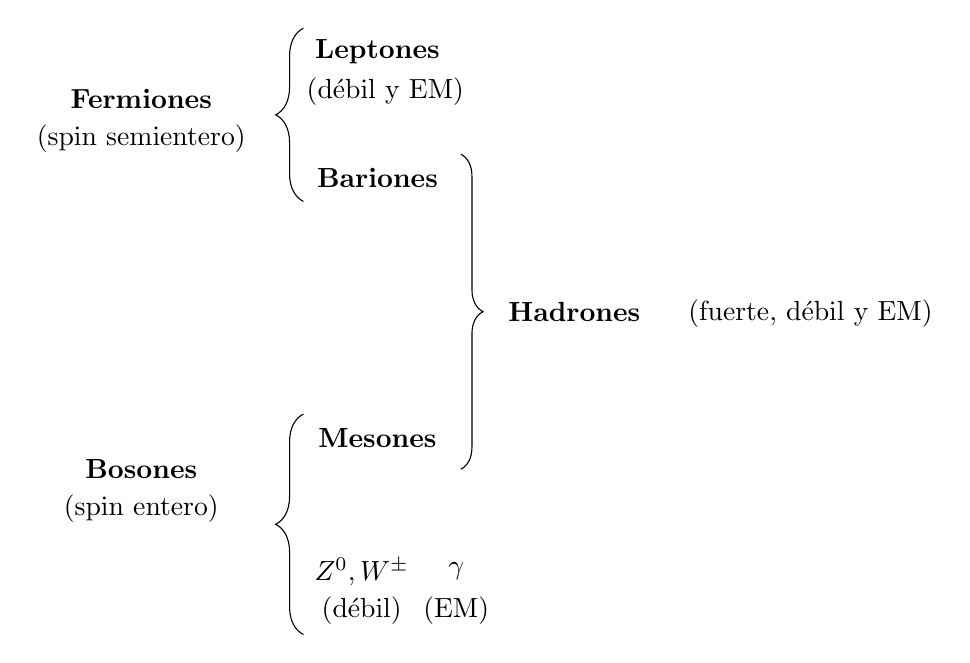
\begin{tikzpicture}

% Fermiones (spin semientero)
\node at (-7,3.5) {\textbf{Fermiones}};
\node at (-7,3) {(spin semientero)};
\draw [decorate,decoration={brace,amplitude=10pt,mirror},xshift=-4pt,yshift=0pt] (-4.8,4.4) -- (-4.8,2.2) node [black,midway,xshift=-1.6cm] {};

% Leptones
\node at (-4,4.1) {\textbf{Leptones}};
\node at (-3.9,3.6) {(débil y EM)};

% Hadrónes (barra de llaves)
\draw [decorate,decoration={brace,amplitude=8pt},xshift=-4pt,yshift=0pt] (-2.8,2.8) -- (-2.8,-1.2) node [black,midway,xshift=1.5cm] {};
\node at (-4,2.5) {\textbf{Bariones}};


% Bariones y Mesones
\node at (-1.5,0.8) {\textbf{Hadrones}};
\node at (1.5,0.77) {(fuerte, débil y EM)};
\node at (-4,-0.8) {\textbf{Mesones}};

% Bosones (spin entero)
\node at (-7,-1.2) {\textbf{Bosones}};
\node at (-7,-1.7) {(spin entero)};
\draw [decorate,decoration={brace,amplitude=10pt,mirror},xshift=-4pt,yshift=0pt] (-4.8,-0.5) -- (-4.8,-3.3) node [black,midway,xshift=-1.6cm] {};

% Fotón y Z0, W±
\node at (-3,-2.5) {$\gamma$};
\node at (-3,-3) {(EM)};
\node at (-4.2,-2.5) {$Z^0, W^\pm$};
\node at (-4.2,-3) {(débil)};
\end{tikzpicture}
\end{figure}
Hay que fijarse que no tenemos quarks ni gluones, esto se debe a que no existen a bajas energía sin estar agregados.

\subsection{Estados excitados}
\noindent
\begin{minipage}{0.6\textwidth} % 60% del ancho del texto para el texto
    \noindent Como hemos visto los bariones en el estado fundamental pueden terner spin $1/2$ y $3/2$, pero por no ser partículas fundamentales se pueden excitar. Si nos fijamos en la ecuación de Schrödinger en tres dimensiones, el término del potencial es
\begin{equation}
    \frac{\hbar^2\ell(\ell+1)}{2\mu r^2}+V(r)
\end{equation}
Los estados fundamentales se dan cuando $\ell=0$ mientras que sí aumentamos $\ell>0$, a distancias cada vez más cercanas a 0 donminará el término centrífugo.
\end{minipage}
\hfill
\begin{minipage}{0.35\textwidth} % 35% del ancho del texto para la figura
    \centering
    \includegraphics[]{Diagramas Tema 1/PotEfectCoulomb.pdf}
    \captionof{figure}{El potencial graficado es $V(r)=-\frac{k}{r}$. Para $\ell=0$ está representado en rojo; y para $\ell=1$ está representado en azul.}
    \label{fig:Sistema dos cuerpos ligados} 
\end{minipage}
\\\\
Se han detectado una cantidad ingente de estados excitados para todo tipo de bariones y mesones como podemos ver en los resúmenes del \href{https://pdg.lbl.gov/2024/tables/contents_tables_baryons.html}{\textit{particle}}.
\section{Antipartículas}
La interacción radiación-materia presenta tres efectos conocidos de menos a más energéticos: fotoeléctrico (orden de los eV), Compton (orden de los Kev) y producción de pares partícula-antipartícula (orden de los MeV), un ejemplo de este último efecto se da cuando un fotón nos genera un par electrón positrón
\begin{equation}
    \gamma \longrightarrow e^-+e^+
\end{equation}
Como idea general las antipartículas tienen la misma masa que sus partículas conjugadas, por lo tanto si nos fijamos en la tabla \ref{tab: Particulas elementales} la masa del electrón es de $\unit[0.51]{MeV}$ por lo que el fotón ha de tener una energía de $\sim\unit[1.2]{MeV}$. Este fenómeno no se puede entender desde el punto de vista de la mecánica cuántica no relativista
\subsection{Mecánica cuántica no relativista}
Vamos a estudiar una partícula libre en el límite no relativista, como sabemos la energía de una partícula libre es  
\begin{equation*}
    E=\frac{p^2}{2m}
\end{equation*}
Por otro lado la información de un sistema físico viene dada por la función de onda $\Psi(\vec{r},t)$ o en el espacio de momentos $\phi(\vec{p},t)$, recordamos que ambas funciones están definidas en el cuerpo $\mathds{C}$. Además hemos de recordar el postulado de la mecánica cuántica que nos asocia a cualquier observable físico un operador hermítico.\\\\
Dicho todo esto vamos a cuantizar $E$ y $\vec{p}$, por lo tanto a estos dos observables les asociamos los siguientes operadores
\begin{equation}
    E\xrightarrow[]{} i\hbar\pdv{}{t} \quad \quad \vec{p} \xrightarrow[]{} -i\hbar \grad
    \label{eq: primera cuantizacion}
\end{equation}
Y podemos construir la ecuación de Schrödinger dependiente del tiempo para una partícula libre 
\begin{equation}
    i\hbar\pdv{\Psi(\vec{r},t)}{t}= -\frac{\hbar}{2m}\grad^2\Psi(\vec{r},t)
    \label{eq: Ec Schrodinger}
\end{equation}
Si nos fijamos esta ``ecuación de ondas'' es en realidad una ecuación del calor ya que el término es de primer orden en la derivada temporal. Decimos que no es una ecuación relativista por \textbf{no ser invariante Lorentz}, es decir, no cumple finitud de la velocidad de la luz.
\noindent
\begin{minipage}{0.6\textwidth} % 60% del ancho del texto para el texto
\subsubsection{Ecuación de continuidad. Implicaciones físicas y matemáticas}
    \noindent Físicamente implica que podemos definir una densidad de probabilidad $\rho(\vec{r},t)=\abs{\Psi(\vec{r},t)}^2$ y por lo tanto la probabilidad la definimos como 
\begin{equation}
    \rho(\vec{r},t)\dd^3 r=\Psi^*(\vec{r},t)\Psi(\vec{r},t) \dd^3 r
\end{equation}
Queremos estudiar cómo varía la probabilidad de encontrar una partícula en un volumen $V$ del espacio en el tiempo.
\end{minipage}
\hfill
\begin{minipage}{0.35\textwidth} % 35% del ancho del texto para la 
    \centering
    \includegraphics[]{Diagramas Tema 1/VariacionProb.pdf}
    \captionof{figure}{Esquema de la variación de probabilidad}
    \label{fig:Sistema dos cuerpos ligados} 
\end{minipage}
\begin{equation}
    \begin{aligned}
        &\pdv{}{t}\int_V\Psi^*(\vec{r},t)\Psi(\vec{r},t) \dd^3 r=-\frac{i\hbar}{2m} \int_V \Psi^*(\vec{r},t)\grad^2\Psi(\vec{r},t)-\qty(\grad^2\Psi^*(\vec{r},t))\Psi(\vec{r},t) \dd^3r\\ & =-\frac{i\hbar}{2m} \int_V \div{\qty[\Psi^*(\vec{r},t)\grad \Psi(\vec{r},t)-\Psi(\vec{r},t)\grad \Psi^*(\vec{r},t)]} \dd^3r=-\frac{i\hbar}{2m} \int_V \div{\vec{j}}\,  \dd^3r=\int_S \vec{j}(\vec{r},t)\cdot  \vec{n}\, \dd S
    \end{aligned}
\end{equation}
En este desarrollo hemos utilizado para la primera igualdad la ecuación de Schrödinger, en la segunda hemos integrado por partes y en la última hemos utilizado el teorema de Gauss. Como vemos el vector tangencial $\vec{\tau}$ no contribuye a la variación del vector flujo $\vec{j}$.\\\\
Con esto podemos construir la \textbf{ecuación de continuidad}
\begin{equation}
    \int_V \pdv{\rho\qty(\vec{r},t)}{t}+ \div{\vec{j}(\vec{r},t)}\, \dd^3r=0 \Rightarrow \pdv{\rho\qty(\vec{r},t)}{t}+ \div{\vec{j}(\vec{r},t)}=0
    \label{eq: Ecuacion de continuidad}
\end{equation}
En resumen la densidad de probabilidad y el vector flujo tienen por
\begin{equation}
\begin{aligned}
    &\rho(\vec{r},t) =\Psi^*(\vec{r},t)\Psi(\vec{r},t)\\
    &\vec{j}(\vec{r},t)=-\frac{i\hbar}{2m} \qty[\Psi^*(\vec{r},t)\grad \Psi(\vec{r},t)-\Psi(\vec{r},t)\grad \Psi^*(\vec{r},t)]
\end{aligned}
\end{equation}

Por otro lado la función de onda para una partícula libre es bien conocida
\begin{equation}
    \Psi(\vec{r},t)=N \exp{i\qty(\vec{r}\cdot \vec{p}-E\cdot t)/\hbar}
    \label{eq: Ecuacion de onda part libre}
\end{equation}
Y como caso particular la densidad de probabilidad y el flujo tienen la expresión
\begin{equation}
    \rho(\vec{r},t)=\abs{N}^2 \quad \quad \vec{j}(\vec{r},t)=\frac{\vec{p}}{m} \abs{N}^2
\end{equation}
Como vemos la densidad de probabilidad es \textbf{adimensional}, mientras que el vector flujo tiene unidades de \textbf{velocidad} \footnote{en unidades naturales también es adimensional}.
\\\\
Como hemos mencionado anteriormente, la ecuación de Schrödinger no es invariante Lorentz, por lo que aún no puede explicar la naturaleza cuántica de los fotones.
\newpage
\subsubsection{¿Por qué no es invariante Lorentz?}
Como sabemos la energía de una partícula viene dada por la expresión
\begin{equation}
    E^2=p^2c^2+m^2c^4 \Rightarrow E=\sqrt{p^2c^2+m^2c^4}
    \label{eq: Energia relativista}
\end{equation}
Desarrollando en serie de Taylor obtenemos
\begin{equation}
    E=\sqrt{p^2c^2+m^2c^4}=mc^2 \sqrt{1+\frac{p^2}{m^2c^4}}= mc^2 \qty[1+\frac{1}{2} \frac{p^2 c^2}{m^2c^4}+\mathcal{O}(p^4)]\approx mc^2+\frac{p^2}{2m}
\end{equation}
Y recuperamos la expresión para la energía cinética no relativista $T_\mathrm{NR}=\dfrac{p^2}{2m}$, esta expresión solo es una aproximación para el límite $pc \ll mc^2$ \footnote{La expresión siempre válida para la energía cinética es $T=E-mc^2$.}.

\subsection{Mecánica cuántica relativista}
De manera análoga a lo que hemos hecho para construir la ecuación de Schrodinger, lo vamos a hacer con la energía relativista 
\begin{equation}
    E^2=p^2c^2+m^2c^4
\end{equation}
Utilizando la cuantización \ref{eq: primera cuantizacion}, obtenemos la ecuación de Klein-Gordon
\begin{equation}
 -\frac{\hbar^2}{c^2}\frac{\partial^2 \Psi(\vec{r},t)}{\partial t^2} = - \hbar^2 \grad^2 \Psi(\vec{r},t) + m^2 c^2 \Psi(\vec{r},t)
 \label{eq: Ecuacion de Klein-Gordon}
\end{equation}
Como vemos esta ecuación es de segundo orden en las derivadas temporales y espaciales, esta ecuación sí considera la finitud de la velocidad de la luz, debido a su invarianza Lorentz. 
\subsubsection{Ecuación de continuidad}
Procediendo de manera similar a como hicimos en la ecuación de Schrödinger, obtenemos la ecuación de continuidad $$\pdv{\rho\qty(\vec{r},t)}{t}+ \div{\vec{j}(\vec{r},t)}=0$$
Con la densidad y el flujo con la forma
\begin{equation}
    \begin{aligned}
            &\rho(\vec{r},t) =\frac{i\hbar}{c^2}\qty[\Psi^*(\vec{r},t)\pdv{\Psi(\vec{r},t)}{t}-\Psi(\vec{r},t)\pdv{\Psi^*(\vec{r},t)}{t}]\\
    &\vec{j}(\vec{r},t)=-i\hbar \qty[\Psi^*(\vec{r},t)\grad \Psi(\vec{r},t)-\Psi(\vec{r},t)\grad \Psi^*(\vec{r},t)]
    \end{aligned}
\end{equation}
Recuperando el caso particular de la partícula libre la densidad y el flujo son 
\begin{equation}
    \rho(\vec{r},t)=2\abs{N}^2\frac{E}{c^2} \quad \quad \vec{j}(\vec{r},t)=2 \abs{N}^2 \vec{p}
    \label{eq: dens prob y flujo K-G}
\end{equation}
En este caso la densidad de probabilidad tiene unidades de masa, y el flujo de momento, lo cual no tiene ningún sentido físico pues la densidad de probabilidad ha de ser adimensional. La ventaja de que estemos trabajando con una ecuación invariante Lorentz es que podemos dividir por cualquier invariante que dejará invariante dichos sistema, en este caso si dividimos por la masa obtendremos un resultado dimensionalmente correcto.
\newpage
\subsubsection{¿Cómo sabemos que la ecuación de Klein-Gordon es covariante Lorentz?}
Hasta ahora hemos hecho una afirmación un poco al aire, al deducir la ecuación de Klein-Gordon de la energía relativista, para demostrar que es covariante Lorentz vamos a calcular los invariantes Lorentz.\\\\
Utilizando la métrica $g^{\mu \nu}=\text{diag}(1, -1, -1, -1)$ el producto escalar de dos vectores $A_\mu, B_\nu$ será $$g^{\mu \nu}A_\mu B_\nu=A_\mu B^\mu=A_0B^0-\vec{A}\vec{B}$$
Si definimos el vector de coordenadas y el vector cuadrimomento como
\begin{equation}
\left. 
    \begin{aligned}
      &x_\mu \equiv (ct,\vec{x})\\
      &p_\mu \equiv \qty(\frac{E}{c},\vec{p})
    \end{aligned}
    \right\} \Rightarrow 
    \begin{aligned}
        &x_\mu x^\mu= c^2t^2-\vec{x}^2 \\
        &p_\mu p^\mu=\frac{E^2}{c^2}-\vec{p}^2=m^2c^2
    \end{aligned}
\end{equation}
Podemos definir el operador cuadrigradiente como 
\begin{equation}
    \partial^\mu \equiv \qty(\frac{\hbar}{c}\pdv{}{t},-\hbar \grad)\Rightarrow \p^\mu\p_\mu=\frac{\hbar^2}{c^2}\pdv[2]{}{t}-\hbar \grad^2 \equiv \square^2
\end{equation}
Por lo que hemos definido así el operador D'Alambertiano. Este operador nos permite escribir escribir la ecuación de Klein-Gordon (\ref{eq: Ecuacion de Klein-Gordon}) en notación convariante
\begin{equation}
    \qty(\frac{\hbar^2}{c^2}\frac{\partial^2}{\partial t^2} - \hbar^2\grad^2) \Psi(\vec{r},t)+m^2 c^2 \Psi(\vec{r},t)=(\square^2+m^2 c^2)\Psi(\vec{r},t)=0
\end{equation}
La función de ondas también es covariante Lorentz ya que la podemos escribir como
\begin{equation}
    \Psi(t,\vec{r})=\Psi(x_\mu)=N\exp{-i\qty(x_\mu p^\mu)/\hbar} 
    \label{eq: Ecuacion de onda part libre covariante}
    \footnotemark
\end{equation}
\footnotetext{El menos es para tener consistencia con la ecuación \ref{eq: Ecuacion de onda part libre}}
\noindent Además definimos el cuadrivector $J_\mu=(c\rho(x_\mu),\vec{j}(x_\mu))=2\abs{N}^2 (\dfrac{E}{c},\vec{p})=2\abs{N}^2 p_\mu$ lo que nos permite escribir la ecuación de continuidad como $\p^\mu J_\mu=0$ con lo que hemos conseguido que todo sea \textbf{covariante Lorentz}.
\subsubsection{Problemas de la ecuación de Klein-Gordon}
La ecuación de Klein-Gordon presenta problemas, estos están en la expresión de la energía relativista
\begin{equation}
    E^2=p^2c^2+m^2c^4 \Rightarrow E= \pm \sqrt{p^2c^2+m^2c^4}
    \label{eq: Energia relativista}
\end{equation}
La existencia de que una de estas soluciones sea negativa nos genera dos problemas
\begin{itemize}
    \item Si nos fijamos en la ecuación de la densidad de probabilidad \ref{eq: dens prob y flujo K-G}, tenemos que existen $\rho(\vec{r},t)<0$, lo que contradice totalmente la interpretación de Heissenberg.
    \item  Para la partícula libre tenemos energías negativas no acotadas inferiormente, por lo que \textbf{no existe un estado fundamental}, esto implica que una partícula estaría decayendo infinitamente.
\end{itemize}
\newpage
\subsubsection{¿Cómo se solucionó dicho problema?}
Si pensamos en el proceso $\gamma \longrightarrow e^-+e^+$, vemos que \textbf{no} se conserva el número de partículas, la conservación del número de partículas es una consecuencia de la mecánica cuántica no relativista.\\\\
Pero sí que tenemos cantidades que se conservan independientemente del marco en el que estemos trabajando, como es el caso de la \textbf{carga eléctrica}. Pauli y Weisskopf propusieron una solución simple pero brillante, como la carga eléctrica es covariante Lorentz, si multiplicamos la corriente por dicha corriente, ésta también lo será por lo tanto $$\vec{J_\mu}=-e\, i(\Psi^*\p_\mu\Psi-\Psi\p_\mu\Psi^*)$$
Recordamos de nuevo que tenemos dos soluciones linealmente independientes $E<0$ y $E>0$
\begin{itemize}
    \item La solución $E>0$ tiene carga $Q$.
    \item La solución $E<0$ tiene carga $-Q$. Esta solución representa una partícula con energía positiva $E>0$ pero con carga opuesta, es decir una \textbf{antipartícula}
\end{itemize}
Las funciones de onda de cada partícula están en espacio de Hilbert distitnos, estas funciones son ortonormales debido precisamente a la carga opuesta que presentan. La forma que tenemos de transformar una función de onda en otra es el operador conjugación de carga (paridad).

\subsection{Diagramas de Feymann}
\noindent
\begin{minipage}{0.6\textwidth}
    Si nos situamos en el sistema centro de masas (CM) de una partícula con carga $Q=-e$ tendremos que el vector cuadrimomento es $p_\mu=\qty(\dfrac{E}{c},\vec{0})$ y por lo tanto el vector cuadricorriente será $$J_\mu=-2e\abs{N}^2\qty(\frac{E}{c}, \vec{0})$$
Sin embargo si tenemos carga $Q=e$ la cuadricorriente es $$J_\mu=2e\abs{N}^2\qty(\frac{E}{c}, \vec{0})=-2e\abs{N}^2\qty(-\frac{E}{c}, \vec{0})$$ 
\end{minipage}
\hfill
\begin{minipage}{0.3\textwidth}
    \centering
    \includegraphics[scale=1.3]{Diagramas Tema 1/Feymann-ElePos.pdf}
    \captionof{figure}{Diagrama de Feymann de una creación de pares electrón-positrón.}
    \label{fig: FeyDia elec-posi}
\end{minipage}
    \\\\\\
Si nos fijamos en la propagación de la función de onda de la solución positiva tenemos $\Psi\equiv \exp{-i\qty(\dfrac{E\, t}{\hbar})}$ mientras que para la solución negativa tenemos  $\Psi\equiv \exp{-i\qty(\dfrac{(-E)\, t}{\hbar})}=\exp{-i\qty(\dfrac{E\, (-t)}{\hbar})}$, es decir, las antipartículas se pueden interpretar como partículas que viajan en hacia atras en el tiempo. En los diagramas de Feymann, como el representado en la figura \ref{fig: FeyDia elec-posi}, las líneas fermiónicas han de ser \textbf{continuas} para representar \textbf{procesos reales}.
\newpage
\subsection{Descubrimiento y detección de las antipartículas}
Supongamos que tenemos un generador de partículas cargadas, si tenemos un selector de velocidades sólo las partículas cargadas con la misma energía cinética saldrán hacia el detector, 
\begin{figure}[h]
    \centering
    \includegraphics{Diagramas Tema 1/SelectorVelocidades.pdf}
    \caption{Esquema de un selector de velocidades. Las únicas partículas que pueden pasar son aquellas con la energía cinética adecuada, $v=\frac{E}{B}$, la masa tienen las partículas en el detector lo podemos calcular mediante la expresión $m=rq\frac{B^2}{E}$}
    \label{fig:enter-label}
\end{figure}

La primera antipartícula que se detectó fue en 1933, cuando en una cámara de niebla, se encontró una partícula con carga muy similar a la del protón, pero cuya masa tenía que ser mucho menor (menor que $\unit[10]{MeV}$), con un análisis un poco más detallado se determinó que debía ser una partícula con masa muy similar (igual) a la del electrón pero con carga opuesta, a esta partícula se la bautizó como \textbf{positrón}.\\\\
Los primeros detectores que se construyeron fueron cámaras de niebla, que estaban formadas por un gas sobresaturado (alcohol ó cualquier líquido volátil). Cuando una partícula cargada atraviesa el gas el campo eléctrico de la partícula genera una perturbación que hace que se formen pequeñas gotas (grosor del haz), por lo que cuanto mayor sea la carga de la partícula que atraviesa la cámara mayor será el grosor del haz.\\\\
\begin{minipage}{0.6\textwidth}
\begin{tcolorbox}[colback=airforceblue!20, colframe=airforceblue, title=Ejemplo: Detección de $\gamma \longrightarrow e^-+e^+$ ]
En la siguiente imagen se muestra cómo se detectó en el expariménto hecho por Anderson, una desintegración de un fotón en un electrón y un positrón. \\\\Si nos fijamos, el fotón deja ningun rastro en la cámara de niebla ya que no está cargado, sin embargo, cuando este se desintegra aparecen muy bien diferenciadas dos curvas iguales pero girando en sentido contrario.
\end{tcolorbox}
\end{minipage}
\hfill
\begin{minipage}{0.35\textwidth}
        \centering
    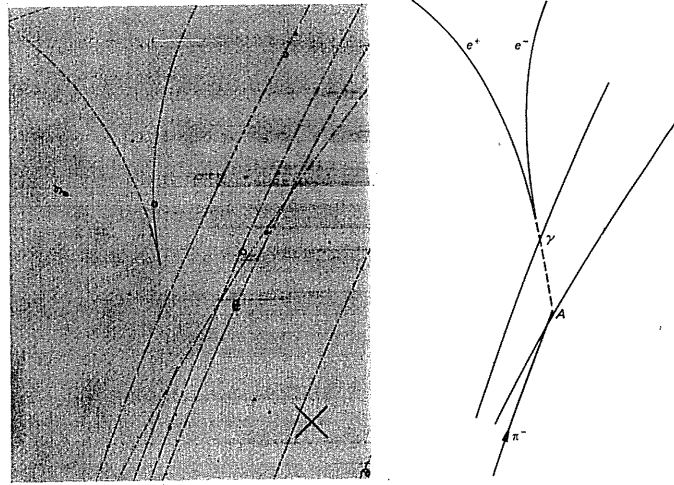
\includegraphics[width=\textwidth]{Imagenes/Camara de niebla.png}
    \captionof{figure}{Desintegración de un fotón en un par electrón-positrón}
    \label{fig: Desint elec-pos}
\end{minipage}
\newpage
\section{Leptones}

\begin{minipage}{0.6\textwidth}
    Como ya hemos mencionado, los leptones son, entre las partículas fundamentales, los fermiones de spin 1/2 que no participan en la interacción fuerte. \\\\
Si nos fijamos, tenemos leptones cargados ($e^-, \mu^-, \tau^-$) y no cargados, los llamados neutrinos. Como los neutrinos no son cargados \textbf{no} pueden participar en los procesos electromagnéticos y sólo participan en procesos \textbf{débiles}, mientras que los leptones cargados participan tanto en procesos electromagnéticos como en débiles.
\end{minipage}
\hfill
\begin{minipage}{0.3\textwidth}
\centering
\begin{tabular}{|c c c|}
\hline
{Nombre}       & {Masa } & {Carga } \\ \hline
$e$                   & 0.511                     & -1                 
\\ 
$\nu_e$    & $<10^{-5}$                & 0                  
\\ \hline
$\mu$                 & 106                       & -1                 
\\ 
$\nu_\mu$             & $<0.2$                    & 0                  
\\ \hline
$\tau$                & 1784                      & -1                 \\ 
$\nu_\tau$            & $<20$                     & 0                  
\\ \hline
\end{tabular}
\captionof{table}{Leptones fundamentales de la materia.}
\label{tab:leptones}
\end{minipage}
\subsubsection{Número leptónico}
A cada una de las familias se les va a asignar un número cuántico conservado, el \textbf{número leptónico}. Cada una de las partículas de una familia tendrán valor +1 mientras que las antipartículas tendrán valor -1.
\begin{tcolorbox}[colback=airforceblue!20, colframe=airforceblue, title=Ejemplo: Conservación del núemero leptónico ]
 Si tenemos la siguiente desintegración$$\gamma \longrightarrow e^-+e^+$$ vemos que el número leptónico al principio de la reacción es nulo, ya que tenemos un fotón mientras que a la derecha, tenemos un +1 que corresponde al electrón y un -1 que corresponde al positrón.\\\\
 La siguiente reacción no podría ser posible
 $$\mu^- \longrightarrow e^- +\gamma$$ ya que no se conservan los números leptónicos, a la izquierda $L_\mu=+1, L_e=0$ y a la derecha $L_\mu=0, L_e=1$, por lo que no se puede dar esta desintegración, la desintegración correcta será $$\mu^- \longrightarrow e^- +\overline{\nu_e}+\nu_\mu$$ Este canal es la manera más probable $\sim 100\%$ que tiene de desintegrarse el muón.
\end{tcolorbox}

El número leptónico se conserva en todos los procesos físico conocidos. Si no exsiten neutrinos en el proceso se reduce a la conservación de pares, por eso los leptones cargados solo pueden crear o destruir pares.
\subsubsection{¿Cómo sabemos que no hay familias de partículas más ligeras que la del electrón?}
Sabemos que no hay más partículas se debe a la estabilidad del electrón, ya que de haberlas, éste tendría que desintegrarse ya que se encontrarían en un estado de energía más bajo.
\newpage
\subsection{Cinemática de partículas cargadas (régimen no relativista)}
Si tenemos una partícula cargada, tiene dos formas de perder energía
\begin{itemize}
    \item \textbf{Colisión elástica}: Una colisión elástica en mecánica cuántica sólo transfiere energía pero no genera nuevos estados. 
    \begin{figure}
        \centering
        \includegraphics[width=0.5\linewidth]{Diagramas Tema 1/ColisionElastica.pdf}
        \caption{Esquema de una colisión elástica. HAY QUE CAMBIARLO}
        \label{fig:Colision Elastica}
    \end{figure}
    De la conservación de la energía y del momento lineal obtenemos
\begin{equation*}
    \begin{aligned}
        &m_1v^2=m_1+u_1^2+m_2u_2^2 \\
        & m_1v_1=m_2u_2 \cos(\phi)+m_1u_1\cos(\theta)\\
        & 0=m_2u_2\sin(\phi)-m_1u_1\sin(\theta)\\
    \end{aligned}
\end{equation*}
Con lo que podemos llegar a la siguiente relación
\begin{equation}
    (m_1+m_2)u_2=2m_1v_1\cos(\phi)
    \label{eq: relacion de transferencia colision elastica}
\end{equation}
Si la energía transferida a la partícula roja, utilizando la relación \ref{eq: relacion de transferencia colision elastica} obtenemos 
\begin{equation}
    \Delta T=\dfrac{1}{2}m_2u_2=\textcolor{red}{\frac{1}{2}} m_2 \frac{4m_1 \textcolor{red}{m_1v_1}}{(m_1+m_2)^2}\cos^2(\phi)= \textcolor{red}{T_\mathrm{i}} \frac{4m_1m_2}{(m_1+m_2)^2} \cos^2(\phi)
\end{equation}
Con lo que podemos obtener el cociente entre la energía transferida respecto a la energía inicial
\begin{equation}
    \frac{\Delta T}{T_\mathrm{i}}=\frac{4m_1m_2}{(m_1+m_2)^2} \cos^2(\phi) 
\end{equation}
Esta transferencia se hace máxima cuando la segunda partícula sale paralela a la trayectoria a la primera, es decir, $\phi=0$. Tenemos dos casos límites
\begin{itemize}
    \item $m_1 \gg m_2$ Para este caso, podemos despreciar $m_2$ en el denominador por lo tanto $\dfrac{\Delta T}{T_\mathrm{i}}=\dfrac{4m_2}{m_1} \xrightarrow[]{}0$, para el caso de un protón y chocando con un electrón $p\xrightarrow[]{}e^-$ la transferencia de energía es del $0.2\%$, esto quiere decir que el protón apenas pierde energía por lo que es muy penetrante.
    \item $m_1\sim m_2$ Para este caso tendremos que la transferencia de energía será \\$\dfrac{\Delta T}{T_\mathrm{i}}=\dfrac{4m_1}{(2m_1)^2} \xrightarrow[]{}1$, para el caso de dos electrones colisionando la transferencia es del $100\%$, por lo que el electrón es muy poco penetrante.
\end{itemize}
     \item \textbf{Radiación de frenado, \textit{Bremsstrahlung}}: Si recordamos cualquier partícula acelerada emite radiación, por lo que cuando una partícula gira, ésta emitirá radiación. Cuando un electrón atraviesa un átomo, recordar que está principalmente vacío, éste interaccionará con el campo electromagnético del átomo \footnote{La contribución principal viene dada por el núcleo}.
     
     \begin{figure}[h]
    \centering
    \includegraphics[]{Diagramas Tema 1/ElectronIntAtomo.pdf}
    \caption{Desviación de una partícula cargada por el campo eléctrico de otra.}
    \label{fig:Desviacion particula}
\end{figure}

     \noindent Si tomamos la expresión no relativista de dicha radiación (fórmula de Larmor)
\begin{equation}
    P=\frac{2}{3}\frac{q^2}{c^3}a^2 \xrightarrow[]{} \qty(\frac{zZ}{m})^2
\end{equation}
Vemos que cuanto mayor masa tenga una partícula menor será la energía emitida por radiación de frenado.

\begin{tcolorbox}[colback=airforceblue!20, colframe=airforceblue, title=Ejemplo: Protón vs electrón]
 Para estudiar las partículas utilizamos aceleradores, si calculamos el cociente entre la masa del protón y la del electrón es $\dfrac{m_p}{m_e}\sim 1900$, el electrón emitirá mucha radiación de frenado mientras que el protón emitirá muy poca, por ello los protones alcanzan energías más altas en los aceleradores de sincrotrón.\\\\
 Como los protones son más penetrantes, son utilizados para tratar tumores de difícil accesibilidad ya que son menos dañinas (aunque más ionizantes), los electrones no traspasan los primeros milímetros de tejido y como transfieren toda su energía provocan mayores daños.
\end{tcolorbox}
Si nos encontramos en el régimen relativista la potencia va como $P\sim m^{-4}$, por lo que se acentúa la diferencia vista en el ejemplo.
\end{itemize}
\subsection{Muones}
Cuando se empezó a estudiar la radiación natural, se pensaba que subiendo en altura detectores disminuiría la radiación ya que se creía que toda provenía del suelo. La sorpresa apareció cuando la radiación no disminuía sino que aumentaba. La radiación que apareció ahora se conocen como \textbf{rayos cósmicos}.
\\\\
Los rayos cósmicos son partículas provenientes del universo que cuando entran en la atmósfera hacen scattering y generan una cascada (\textit{shower}) de partículas hacia la superficie de la Tierra.
\newpage
\begin{figure}
    \centering

    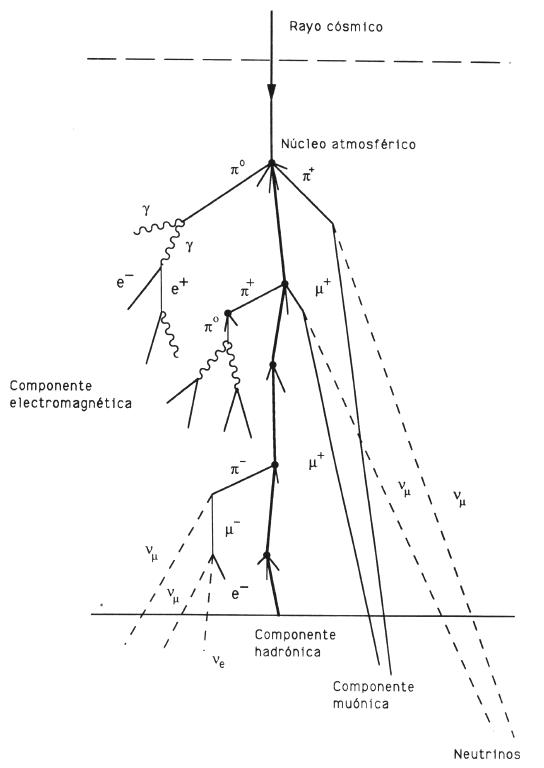
\includegraphics[width=0.85\textwidth]{Imagenes/RayosCosmicos.jpg}
    \caption{Scattering producido por un rayo cósmico. Vemos que se generan cuatro componentes: \textbf{electromagnética}, \textbf{hadrónica}, \textbf{muónica} y \textbf{neutrinos}. La componente electromagnética no atraviesa la atmósfera; de las componentes hadrónicas y muónicas tan sólo nos llegan algunas partículas; los neutrinos atraviesan sin ningún problema tanto la atmósfera como la Tierra.}
    \label{fig: rayo cosmico}
\end{figure}
\clearpage
\subsubsection{Descubrimiento del muón}
    El muón se detectó por primera vez en 1937. Se detectarón a la vez tanto una partícula como una antipartícula. Se teorizó con que se debía a una generación de pares causada por un fotón, aunque el par no era muón-antimuón, sino electrón-positrón pero ambos en un estado excitado.
\subsection{Neutrinos}
Los núcleos atómicos los denotamos como $^A _Z X$, por ejemplo para el plomo 208 tenemos
\begin{itemize}
    \item El número atómico es $Z=82$, que corresponde al número de protones.
    \item  El número de másico es $A=208$, que corresponde a la suma de nucleones dentro del núcleo.
    \item El número de neutrones $N=126$.
\end{itemize}
\begin{figure}[h]
    \centering
    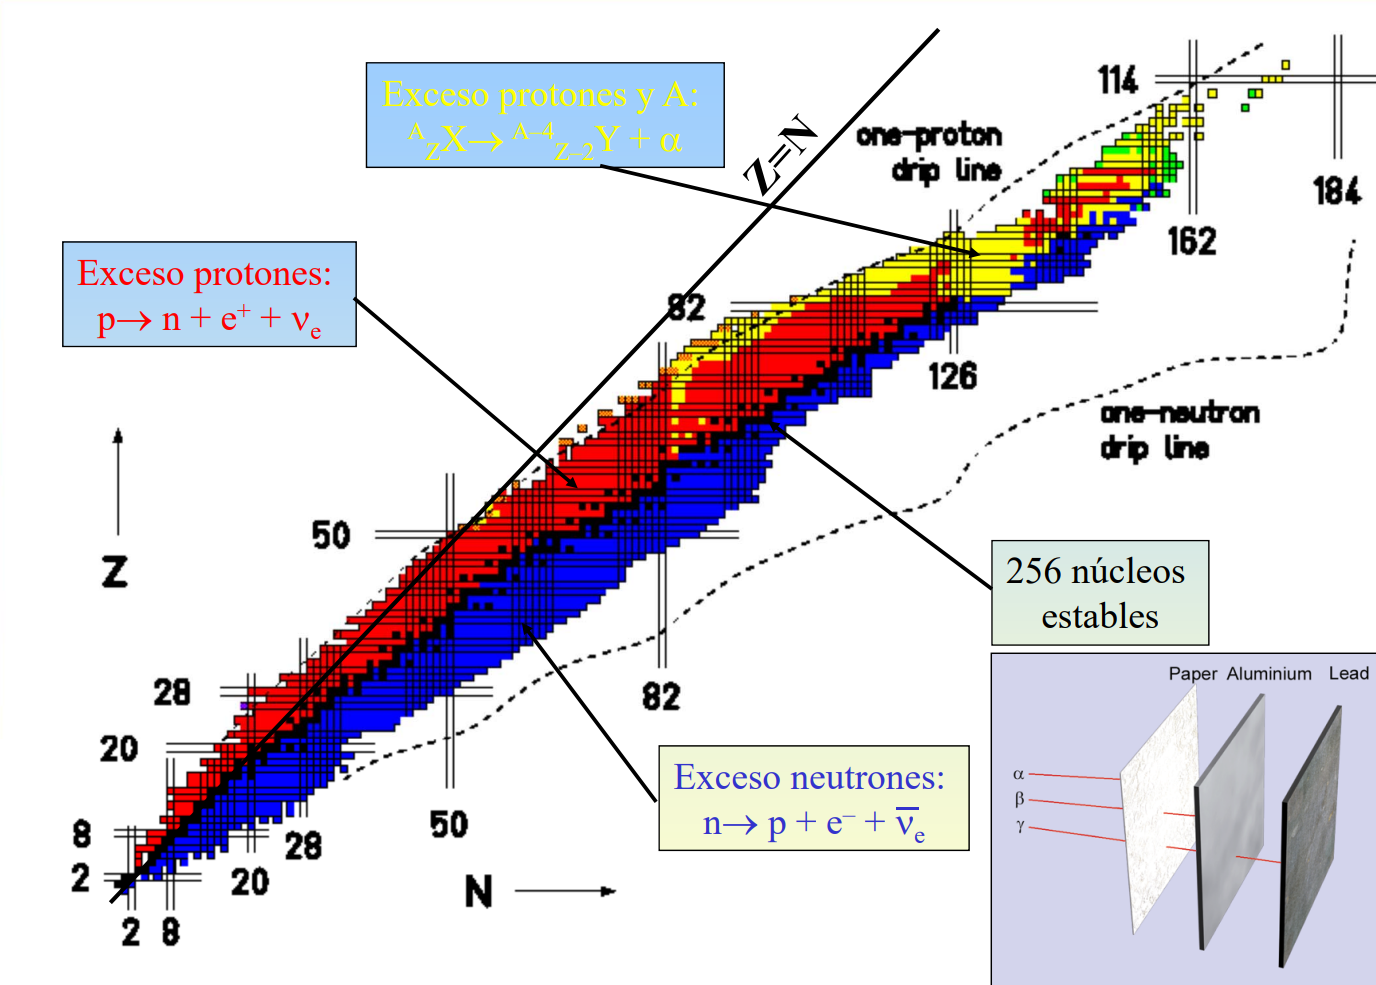
\includegraphics[scale=0.3]{Imagenes/DiagramaSegre.png}
    \captionof{figure}{Diagrama de Segre y capacidad de penetración de los distintos tipos de radiación. La línea negra representa los núcleos con el mismo número de protones y neutrones, la zona azul exceso de neutrones y la zona roja tiene exceso de protones. Las líneas discontinuas se conocen como \textbf{líneas de volteo}, estas líneas encierran la figura por lo que si añadimos por fuera de la inferior un neutrón éste no se ligará, y si añadimos un protón fuera de la superior éste no se ligará.}
    \label{fig: Diagrama Segre}
\end{figure}
Un núcleo puede desintegrarse mediante decaimiento $\beta$. En el diagrama de Segre (figura \ref{fig: Diagrama Segre}), los núcleos de la zona roja se desintegran a partir de decaimiento $\beta^+$, mientras que los que se encuentran en la zona azul tendremos decaimiento $\beta^-$. \footnote{Las partículas entre corchetes es para conservar el número leptónico.}
\newpage
\begin{itemize}
    \item \textbf{Decaimiento $\bm{\beta^-}$}: es la desintegración de un neutrón $n \longrightarrow p+e^-+[x_\nu]$ si tenemos un núcleo $(A,Z) \longrightarrow (A,Z+1)+e^-+[x_\nu]$.
    \item \textbf{Decaimiento $\bm{\beta^+}$}: es la desintegración de un protón $p \longrightarrow n+e^++[y_\nu]$ si tenemos un núcleo $(A,Z) \longrightarrow (A,Z-1)+e^-+[y_\nu]$.
\end{itemize}
Hay otra via para que un protón se transforme en un neutrón, es lo que se conoce como \textbf{captura electrónica}. En un átomo tenemos una posibilidad no nula de encontrar un electrón de la corteza en el núcleo. Cuando esto sucede se da el siguiente proceso $e^-+p\longrightarrow n+[z_\nu]$ y para el núcleo tenemos $e^-+(A,Z) \longrightarrow (A,Z-1)+[z_\nu]$.\\\\
De los decaimiento podemos hacer el estudio a través de las masas de los núcleos
\begin{equation}
    M_1\longrightarrow M_2+m \Rightarrow \Delta M=M_1-M_2-m>0
\end{equation}
En unidades naturales $\Delta M$ es la energía cinética que adquieren tanto $M_2$ como $m$, por lo tanto
\begin{equation*}
    \Delta M=\frac{p^2_{M_2}}{2M_2}+ \frac{p^2_{m}}{2m}
\end{equation*}
Por conservación del momento $\abs{p_{M_2}}=\abs{p_m}$ 
\begin{equation}
    \Delta M=\frac{p^2_{M_2}}{2M_2}+ \frac{p^2_{m}}{2m}=\frac{p^2_{m}}{2m}\qty(1+\frac{m}{M_2})=T_m\qty(1+\frac{m}{M_2})\Rightarrow T_m=\frac{\Delta M}{1+\dfrac{m}{M_2}}
    \label{eq: energia cinetica electron}
\end{equation}
Que para el caso de los decaimientos $\beta^\pm$ de los núcleos todos los valores de las masas son conocidos y son fijos, por lo que $m=m_e\lll M_2$ y  haciendo un desarrollo obtenemos $T_m \simeq \Delta M$, es decir, que la energía cinética del electrón siempre tenía que ser la misma y al ser la partícula más ligera es el que se lleva la mayor parte de la energía cinética.\\

\begin{minipage}{0.6\textwidth}
\begin{tcolorbox}[colback=airforceblue!20, colframe=airforceblue, title=Ejemplo: Desintegración del Bismuto-210]
 Si calculamos la energía que tiene la desintegración del $^{210}\text{Bi}$ en $^{210}\text{Po}$, $M_1=\unit[195600.2]{MeV}, M_2=\unit[195599]{MeV}$, cuya diferencia es de $\unit[1.16]{MeV}$ Por lo que corresponde con el valor que se muestra en la figura \ref{fig: DistribucionElectrones}.\\\\ Al término $\Delta M$ debemos sumarle las aportaciones de las energías de enlace por nucleón y la reionización del átomo para obtener dicha energía.
\end{tcolorbox}
\end{minipage}
\hfill
\begin{minipage}{0.35\textwidth}
    \centering
    \includegraphics[width=\textwidth]{Diagramas Tema 1/DistribucionEnergiaElectrones.pdf}
    \captionof{figure}{Distribución de energía cinética de los electrones}
    \label{fig: DistribucionElectrones}
\end{minipage}\\\\
Pero esto no explicaba que la distribución de energia cinética fuera una suave distribución y no un valor fijo.\\\\
En 1930 Pauli postuló el neutrino, que resolvía el problema de la distribución continua. Y se consiguió detectar en 1956.
\clearpage
\subsubsection{La necesidad del neutrino}
Vamos a analizar la reacción $n \longrightarrow p+e^-$. Si componemos los momentos angulares del protón y del electrón tenemos que componer $\dfrac{1}{2}\otimes \dfrac{1}{2}=0\oplus 1$, es decir, tenemos un bosón. Pero hemos partido de un neutrón, que es un fermión, por lo que si no consideramos que hay una partícula $[x_\nu]$ (como en la ecuacion del decaimiento $\beta^-$ anterior) no se conservaría el momento angular a escala subatómica y eso no puede ser.\\\\
Necesariamente tenemos que introducir una nueva partícula que ha de ser un \textbf{fermión} de spin $\dfrac{1}{2}$. Por lo que si acoplamos los 3 spines $\dfrac{1}{2}$ obtenemos el mismo resultado que la ecuación \ref{eq: Acoplamiento 3 spines 1/2}. Además como en la ecuación anterior sí que se conserva la carga, debe ser \textbf{neutra} y para que no se pueda su masa debía ser \textbf{muy baja} para ya que debía de estar por debajo de la precisión de los instrumentos. \\\\Posteriormente, con la incorporación de los números cuánticos, se determinaría que esta partícula debía ser una antipartícula, como ya denotamos a continuación. \footnote{Estamos introduciendo al neutrino como lo conocemos ahora aunque todavía no hemos determinado si el neutrino tiene antipartícula o no ó si es o no único.}
\subsubsection{Reacciones permitidas y no permitidas}
En toda la sección hemos planteado que el decaimiento $\beta^\pm$ se da en núcleos, pero, ¿se dará si tenemos al protón y al neutrón libres?\\\\
Recordemos que el decaimiento $\beta^-$ es la reacción
\begin{equation}
    n\longrightarrow p+e^-+\overline{\nu_e}
    \label{eq: Decaimiento beta -}
\end{equation}
Mientras que el decaimiento $\beta^+$ es la reacción
\begin{equation}
    p \longrightarrow n+e^++\nu_e
    \label{eq: Decaimiento beta +}
\end{equation}
En la naturaleza no sólo tenemos constricciones en los procesos con los números cuánticos y la carga, sino que también tenemos las ligaduras ``clásicas'': energía, momento lineal, momento angular...\\\\
La reacción \ref{eq: Decaimiento beta -} sí que se puede dar en partículas libres ya que conserva carga, número leptónico y energía, como $m_n-m_p\approx \unit[1.3]{MeV}$, si que nos cabe el electrón. Sin embargo para la reacción \ref{eq: Decaimiento beta +} aunque se conservan la carga y el número leptónico, no se conserva la energía y por eso no está permitida para protones libres.\\\\
Para ``pasar'' en reacciones de un lado a otro de la flecha, necesitamos conjugar la partícula. Por lo tanto de la racción \ref{eq: Decaimiento beta +} obtenemos otra reacción permitida
\begin{equation}
    \overline{\nu_e} + p \longrightarrow n+e^+
    \label{eq: colision proton antineutrino}
\end{equation}
En las colisiones, no tenemos problemas físicos con la energía ya que siempre puede alcanzarse en forma de energía cinética.
\clearpage
\subsubsection{Descubrimiento del neutrino}
En 1930, Hans Bethe propuso una forma de detectar los neutrinos, éstos se habían de detectar de manera indirecta. El procedimiento es el siguiente, mediante una colisión entre un antineutrino y un protón se generan un neutrón y un positrón
\begin{equation}
    \overline{\nu_e} + p \longrightarrow n+e^+
\end{equation}
Ese positrón se aniquila con un electrón dando lugar a un par de fotones, para que se conserve el momento lineal ambos saldrán en direcciones contrarias.
\begin{equation}
    e^++e^-\longrightarrow \gamma + \gamma
    \label{eq: aniquilacion e+ e-}
\end{equation}
Y el neutrón que se genera ha de ser capturado por otro núcleo liberando un fotón, correspondiente a la energía de ligadura.
\begin{equation}
    n+^A_ZX\longrightarrow ^{A+1}_Z X+ \gamma
    \label{eq: captura neutronica}
\end{equation}
En un proceso que se conoce como \textbf{captura neutrónica}.\\\\
Fue así como en 1956 Reines, Clyde y Cowan descubren el neutrino, para ello se fueron a un reactor nuclear, que es un generador de antineutrinos; y colocaron un tanque con agua al lado, después disolvieron en agua una sal de cadmio\footnote{El cadmio tiene una sección de captura neutrónica muy grande.} $(\text{CdCl}_2)$ y observaron primero dos fotones emitidos en direcciones opuestas a la vez y poco después varios fotones
\begin{figure}[h]
\begin{subfigure}[h]{0.45\textwidth}
    \centering
    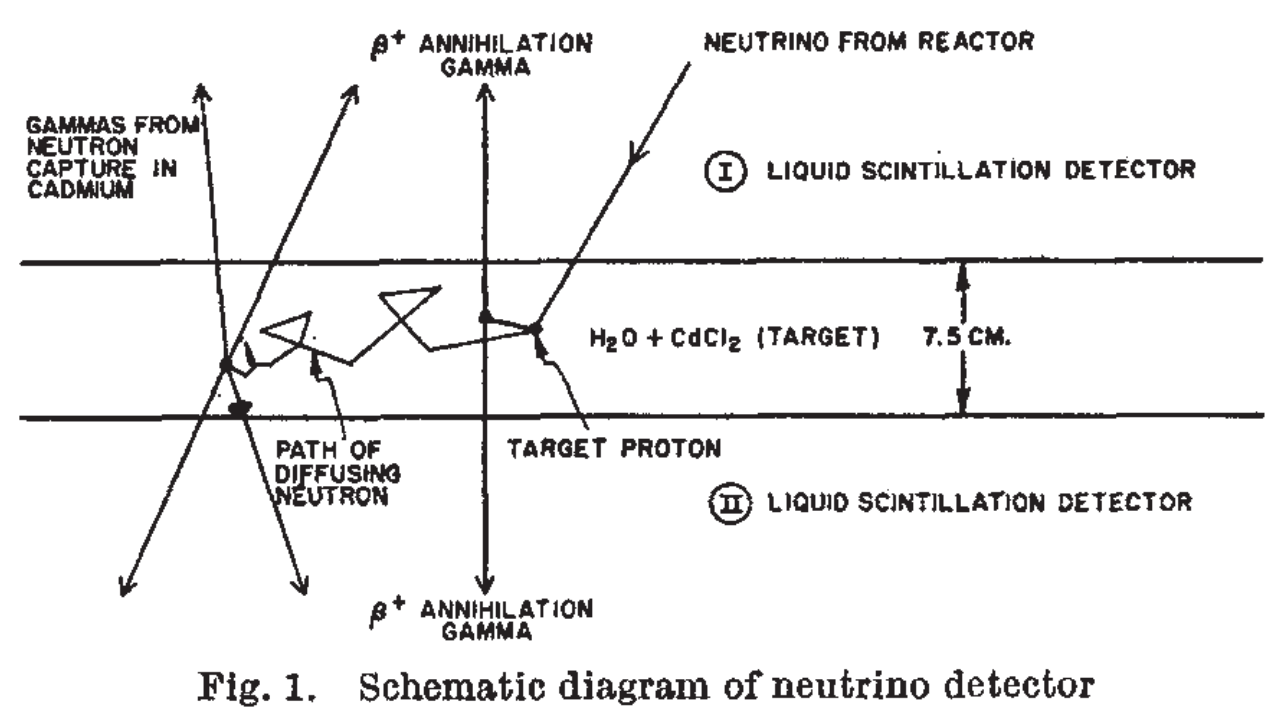
\includegraphics[width=\textwidth]{Imagenes/ExperimentoNeutrino.png}
    \subcaption{Esquema del experimento de detección de neutrinos}
\end{subfigure}
\hfill
\begin{subfigure}[h]{0.45\textwidth}
    \centering
    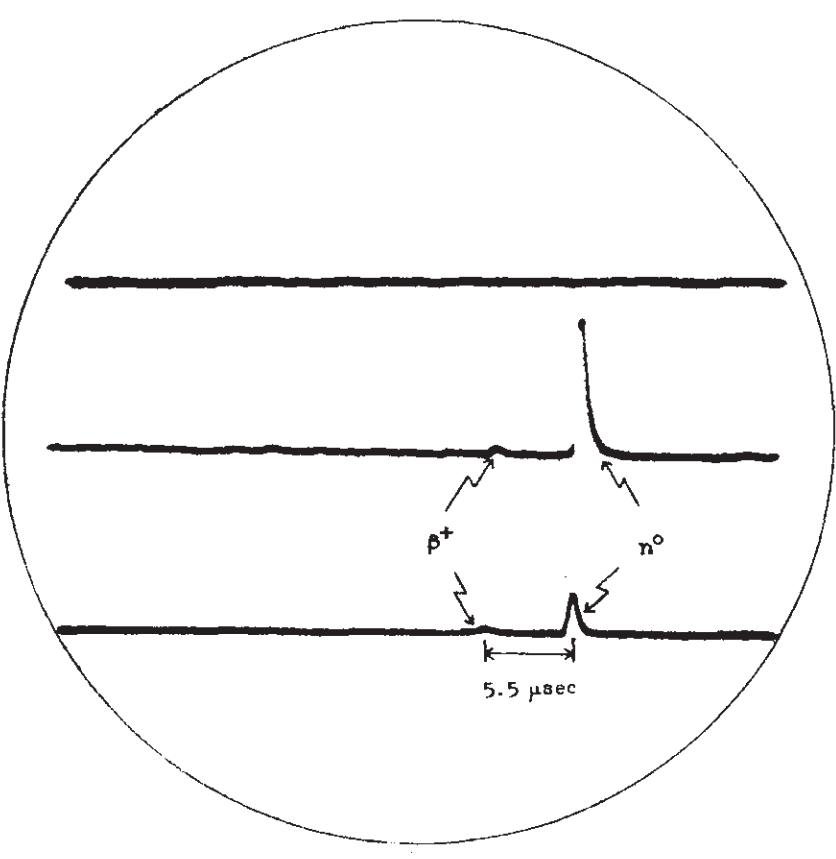
\includegraphics[scale=0.3]{Imagenes/DeteccionNeutrino.png}
    \subcaption{Esquema de la detección del neutrino. \textit{Foto más maravillosa y perfecta de un neutrino.}}
\end{subfigure}
\caption{Diseño del experimento y señal del neutrino. Aunque en la segunda imágen no se aprecia, hay un intervalo entre la primera detección de fotones y la segunda de $\unit[5.5]{\mu s}$, además se detectan dos fotones con diferentes energías al contrario que los detectados por la aniquilación de pares.}
\end{figure}

\noindent Ahora queda estudiar si el neutrino es único, es decir, es sólo perteneciente a una familia, y si tiene no una antipartcula.\\\\
\newpage
\subsubsection{¿Tiene el neutrino antipartícula?}
De los experimentos de Raines y Cowan se obtienen como productos la reacción \ref{eq: colision proton antineutrino}
\begin{equation*}
    \overline{\nu_e} + p \longrightarrow n+e^+ \quad \text{pero no} \quad \nu_e+n\longrightarrow p+e^-
\end{equation*}
Si se diera la segunda reacción tendríamos que los neutrinos interaccionan por de la misma manera con los nucleones del núcleo.
En 1955 se realizó un experimento que se basaba en la siguiente reacción
\begin{equation}
    \nu_e+^{37}_{17}\text{Cl}\longrightarrow e^-+^{37}_{18}\text{Ar}
\end{equation}
Como el Argón tiene un tiempo de vida medio de 35 días, si se producía la reacción debía haber cantidades considerables de Ar.  Si el experimento resultaba positivo el neutrino debía ser igual a su antipartícula y si resultaba negativo no lo eran. Para ello se midieron las reacciones que producían la radiación cósmica y solar sobre un tanque de cloro. Después se enterró el tanque y las reacciones de Ar que se producían eran de la sensibilidad del medidor por lo que se determinó que \textbf{no} eran la misma partícula.
\subsubsection{¿Existen más tipos de neutrinos?}
Así como se determinó que el muón tenía propiedades análogas a las del electrón pero con mayor masa (e inestabilidad), en los años 60 ya había dado tiempo para caracterizar las propiedades del muón (descubierto 30 años antes). \\\\
A finales de los 50 se descubrieron los piones, $\pi^\pm,\pi^0$, los piones tienen un tiempo de desintegración de $\tau\sim \unit[10]{ns}$, los piones decaen en muones a través de
\begin{equation}
    \pi^\pm \longrightarrow \mu^\pm +\nu/\overline{\nu}
    \label{eq: desintegracion piones}
\end{equation}
Para ello se desarrolló un experimento en Brookhaven que consistía en acelerar protones a velocidades ultrarrelativistas.

\begin{figure}[h]
    \centering
    \includegraphics[]{Diagramas Tema 1/ExpBrookhaven.pdf}
    \caption{Esquema del experimento de Brookhaven.}
    \label{fig:ExpBrookhaven}
\end{figure}
Si el neutrino fuera único, es decir, que el producido por desintegración de piones y por decaimiento beta fuera el mismo; en el régimen ultrarrelativista se debían poder dar más o menos la misma proporción de reacciones.
\begin{equation}
\left.
    \begin{aligned}
        & \overline{\nu}+p \longrightarrow n+e^+  \\
    & \nu+n \longrightarrow p+e^-
    \end{aligned}
    \hspace{1cm}
\right\|
\hspace{1cm}
\begin{aligned}
    & \overline{\nu}+p \longrightarrow n+\mu^+ \\
     & \nu+n \longrightarrow p+\mu^-
\end{aligned}
\label{eq: creacion de leptones carados}
\end{equation}
Vamos a explicar la figura \ref{fig:ExpBrookhaven}.  Un haz de protones con una energía cinética de $\unit[15]{GeV}$ choca contra una lámina de berilio generando piones. Estos piones recorren una distancia de $\unit[21]{m}$ hasta llegar al colimador, a lo largo de esta distancia el pion ya se ha desintegrado y hemos obenido muones y neutrinos. Los muones al llegar al detector, compuesto por un bloque de aluminio y un detector de partículas cargadas, han dejado su energía en los primeros $\unit[25]{cm}$ de longitud. Con lo cual los neutrinos debían dar lugar a las reacciones de la ecuación\ref{eq: creacion de leptones carados}, como sólo se detectaban muones, se concluyó que el neutrino no era único sino que había neutrinos de distintas familias.
\\\\
En los apéndices \ref{chap: Apendice A} y \ref{chap: Apendice B} se detalla toda la física necesaria para entender la producción y detección de las partículas más pesadas.
\subsection{La familia Tau}
En 1975 se detectó una pérdida de energía en un scattering de un par electrón-antielectrón,
\begin{equation}
    e^-+e^+\longrightarrow e^\pm +\mu^\mp + \geq \ \text{2 partículas no detectadas}
\end{equation}
Por conservación de carga se determinó que las partículas debían ser cargadas y que se produjeron por pares, como en los electrones y los muones. Cuando se midió la sección eficaz de los eventos se observó un pico como los que encontramos en la figura \ref{fig:Resonancias en seccion eficaz}  %INTRODUCIR LA IMAGEN DE LA SECCIÓN EFICAZ DEL PAPAER DE 1975
Después de un análisis estadístico (bastante pobre pues se hizo estadística con 8 eventos únicamente) se determinó que la masa de las nuevas partículas debía estar entre $\unit[1.6]{GeV/\textit{c}^2}$ y $\unit[2]{GeV/\textit{c}^2}$.
\\\\
Esta hipótesis resultó correcta pues si nos fijamos en la tabla \ref{tab: Particulas elementales} la masa del tau es de $\unit[1784]{GeV/\textit{c}^2}$
\subsubsection{Neutrino Tau}
Como el resto de familias de leptones tenían un neutrino asociado, se sabía que el tau debía tener un neutrino de su misma familia. No fue hasta el año 2001 que se pudo detectar una interacción del nautrino tau. Aunque el experimento realizado era análogo al realizado para la detección de los neutrinos electrónico y muónico, al ser el $\tau$ una partícula tan inestable, no se podía detectar ya que apenas recorría $\unit[2]{mm}$ antes de decaer. Se detectaron 4 eventos: 2 a través del canal
\begin{equation}
    \tau^- \longrightarrow e^-+\nu_\tau+\overline{\nu_e}
\end{equation}
Y otros a través del canal 
\begin{equation}
    \tau^- \longrightarrow h+\nu_\tau+X
\end{equation}
\section{Quarks y hadrones}
Como ya vimos en la sección \ref{subsubsec: Quarks y hadrones} los quarks son fermiones cargados de spin $1/2$ que participan en la interacción fuerte. Como vimos en la tabla \ref{tab: Particulas elementales} se clasifican en 3 familias, los quarks $u$, $c$ y $t$ tienen carga $q=2/3$ mientras que los quarks $d,s$ y $b$ tienen carga $-1/3$, cada uno de ellos tienen a su vez sus propias antipartículas. \\\\ 
Como vemos los quarks no tienen cargas que sean múltiplos enteros de la carga del electrón sino que es fraccionaria, esto hace que en la naturaleza no podamos tener quarks aislados, sino que únicamente podamos tener quarks en agregados de 3 partículas, \textbf{bariones}; o de una partícula y una antipartícula, \textbf{mesones}. De ahí que las masas que aparecene en la tabla \ref{tab: Particulas elementales} sólo se pueda determinar por métodos indirectos.
\subsection{Números cuánticos de los quarks. Sabores}
De manera similar a los leptones, podemos definir números cuánticos para los quarksm, denominados \textbf{sabores}. 
\begin{itemize}
    \item \textbf{Isospín}: Es el sabor asociado a los quarks $u$ y $d$. Asignamos al quark $I(u)=1/2$ y $I(d)=-1/2$ \footnote{En el capítulo 2 veremos que corresponde a la tercera componente de isospín, de momento vamos a quedarnos con el valor absoluto de todo el isospín.}.
    \item \textbf{Extrañeza}: Es el sabor asociado al quark extraño $s$. Se define como $\Tilde{s}=-\qty(N\qty(s)-N\qty(\overline{s}))$.
    \item  \textbf{Encanto}: Es el sabor asociado al quark encantado $c$. Se define como $\Tilde{c}=N\qty(c)-N\qty(\overline{c})$.
    \item \textbf{Belleza}: Es el sabor asociado al quark bottom (bello) $b$. Se define como $\Tilde{b}=-\qty(N\qty(b)-N\qty(\overline{b}))$
\end{itemize}
Todos estos números cuánticos \textbf{se conservan} en procesos \textbf{fuertes} pero \textbf{no se conesrvan} en procesos \textbf{débiles}.
\subsubsection{Número Bariónico}
Todos los quarks tienen un número común, llamado \textbf{número bariónico} $B$. A los quarks se les asigna un número bariónico $B(q)=1/3$ mientras que a los antiquarks se les asigna $B\qty(\overline{q})=-1/3$. Así definimos el número bariónico de un hadrón como \begin{equation}
    B=\frac{1}{3} \qty(N(q)+N\qty(\overline{q}))
\end{equation}
Obteniendo así que los bariones tienen número bariónico 1 y los mesones 0. Este número cuántico \textbf{se conserva} en todos los procesos físicos conocidos. 

\subsection{El zoo de las partículas elementales}
\noindent
\begin{minipage}{0.45\textwidth}
    En las tablas \ref{tab: Bariones} y \ref{tab: Mesones} se recogen las principales características de los mesones y los bariones.\\\\
    Como vemos en la figura \ref{fig: Zoo particulas} tenemos una cantidad ingente de partículas hacia el año 1955. W.Lamb en ese mismo año durante su discurso del nóbel dijo: \textit{Maybe physicists discovering a new particle ought to be fine 10.000}
\end{minipage}
\hfill
\begin{minipage}{0.45\textwidth}
    \centering
    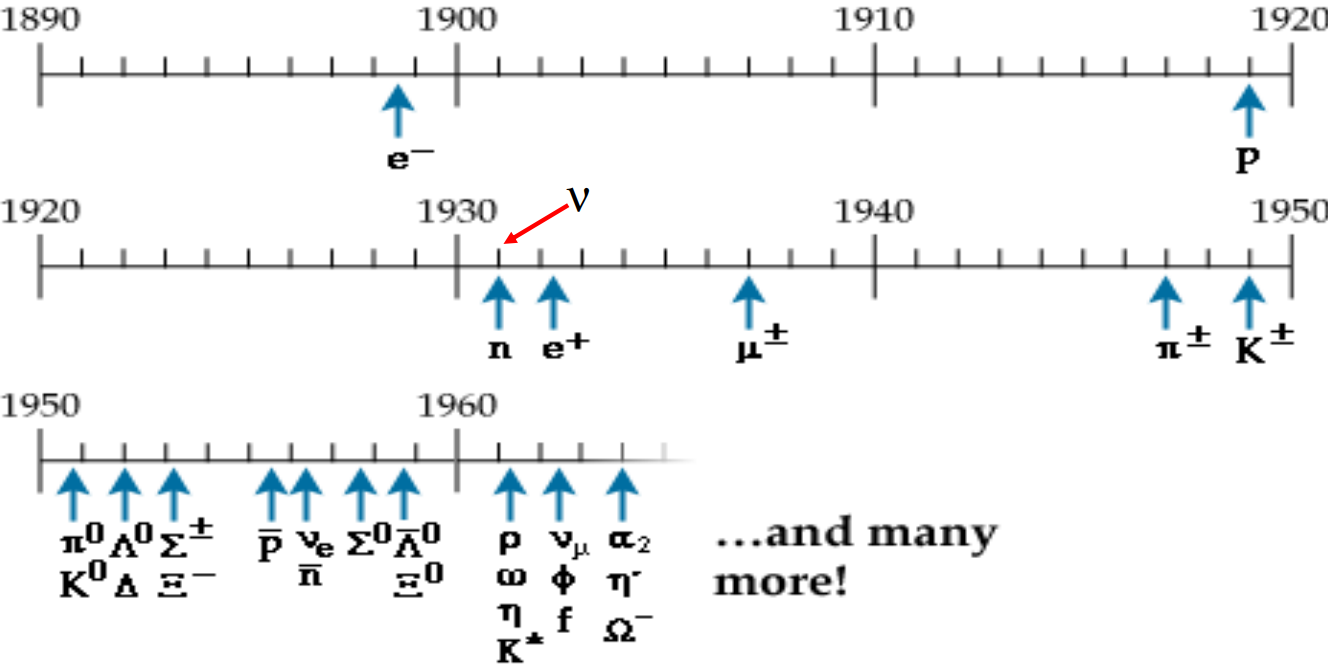
\includegraphics[width=\linewidth]{Imagenes/ParticleZoo.png}
    \captionof{figure}{Línea temporal del descubrimiento de las partículas elementales.}
    \label{fig: Zoo particulas}
\end{minipage}
\begin{table}[h]
    \centering
\begin{tabular}{|c|c|c|c|c|c|c|c|}
\hline
Barión            & $Q$  & Quarks       & $I$    & $\Tilde{s}$ & $\Tilde{c}$ & $\Tilde{b}$ & Masa   \\ \hline
$p^{+}$           & $+1$ & \textit{uud} & $1/2$  & 0           & 0           & 0           & 938.3  \\
$n^{0}$           & $0$  & \textit{udd} & $1/2$  & 0           & 0           & 0           & 939.6  \\
$\Delta^{++}$     & $+2$ & \textit{uuu} & $3/2$  & 0           & 0           & 0           & 1232   \\
$\Delta^{+}$      & $+1$ & \textit{uud} & $3/2$  & 0           & 0           & 0           & 1232   \\
$\Delta^{0}$      & $0$  & \textit{udd} & $3/2$  & 0           & 0           & 0           & 1232   \\  \hline \hline
$\Lambda^{0}$     & $0$  & \textit{uds} & $0$    & -1          & 0           & 0           & 1115.7 \\
$\Sigma^{0}$      & $0$  & \textit{uds} & $1$    & -1          & 0           & 0           & 1192.6 \\
$\Sigma^{+}$      & $+1$ & \textit{uus} & $1$    & -1          & 0           & 0           & 1189.4 \\
$\Sigma^{-}$      & $-1$ & \textit{dds} & $1$    & -1          & 0           & 0           & 1197.4 \\
$\Xi^{0}$         & $0$  & \textit{uss} & $1/2$  & -2          & 0           & 0           & 1314.8 \\
$\Xi^{-}$         & $-1$ & \textit{dss} & $1/2$  & -2          & 0           & 0           & 1321.7 \\
$\Omega^{-}$      & $-1$ & \textit{sss} & $0$    & -3          & 0           & 0           & 1672.5 \\ \hline \hline
$\Lambda_{c}^{+}$ & $+1$ & \textit{udc} & $0$    & 0           & 1           & 0           & 2286.5 \\
$\Sigma_{c}^{0}$  & $0$  & \textit{udc} & $1$    & 0           & 1           & 0           & 2453.8 \\
$\Sigma_{c}^{+}$  & $+1$ & \textit{uuc} & $1$    & 0           & 1           & 0           & 2452.9 \\
$\Sigma_{c}^{++}$ & $+2$ & \textit{uuc} & $1$    & 0           & 1           & 0           & 2453.8 \\
$\Xi_{c}^{0}$     & $0$  & \textit{usc} & $1/2$  & -1          & 1           & 0           & 2470.9 \\
$\Xi_{c}^{+}$     & $+1$ & \textit{dsc} & $1/2$  & -1          & 1           & 0           & 2467.8 \\
$\Omega_{c}^{0}$  & $0$  & \textit{ssc} & $0$    & -2          & 1           & 0           & 2695.2 \\
$\Xi_{c}^{++}$ & $+2$ & \textit{ccu} & $1/2$  & -1          & 2           & 0           & 2766.0 \\
$\Omega_{cc}$  & $+1$ & \textit{ccs} & $1/2$  & -1          & 2           & 0           & 2766.0 \\ \hline \hline
$\Lambda_{b}^{0}$ & $0$  & \textit{udb} & $0$    & 0           & 0           & -1          & 5619.6 \\
$\Sigma_{b}^{-}$  & $-1$ & \textit{ddb} & $1$    & 0           & 0           & -1          & 5815.5 \\
$\Sigma_{b}^{0}$  & $0$  & \textit{udb} & $1$    & 0           & 0           & -1          & 5812.7 \\
$\Sigma_{b}^{+}$  & $+1$ & \textit{uub} & $1$    & 0           & 0           & -1          & 5807.8 \\
$\Xi_{b}^{-}$     & $-1$ & \textit{usb} & $1/2$  & -1          & 0           & -1          & 5791.9 \\
$\Xi_{b}^{0}$     & $0$  & \textit{dsb} & $1/2$  & -1          & 0           & -1          & 5793.1 \\
$\Omega_{b}^{-}$  & $-1$ & \textit{ssb} & $0$    & -2          & 0           & -1          & 6046.1 \\
$\Omega_{b}^{++}$ & $+2$ & \textit{bbq} & $1/2$  & 0           & 0           & -2          & 6100.0 \\
$\Omega_{bb}^{+}$  & $+1$ & \textit{bbq} & $1/2$  & 0           & 0           & -2          & 6100.0 \\
$\Omega_{bbb}^{-}$  & $-1$ & \textit{bbb} & $0$    & 0           & 0           & -3          & 6100.0 \\ \hline
\end{tabular}
\caption{Bariones y sus principales propiedades. La tabla \ref{tab: Bariones} está dividida en 4 cuadrados, cada uno de ellos tiene asociado un sabor, isospín, extrañeza, encanto y belleza, respectivamente.}
\label{tab: Bariones}
\end{table}

\newpage
\begin{table}[h]
    \centering
    \begin{tabular}{|c|c|c|c|c|c|c|c|c|} \hline 
        Mesón & $Q$ & Quarks & $J$ &  \textit{I} & $\tilde{s}$ & $\tilde{c}$ & $\tilde{b}$ & Masa \\ 
        \hline 
        $\pi^{0}$ & $0$ & $u\bar{u} - d\bar{d}$ & 0 & 1 & 0 & 0 & 0 & 134.98 \\ 
        $\pi^{+}$ & $+1$ & $u\bar{d}$ & 0 & 1 & 0 & 0 & 0 & 139.57 \\ 
        $\pi^{-}$ & $-1$ & $d\bar{u}$ & 0 & 1 & 0 & 0 & 0 & 139.57 \\ 
        $\rho^{0}$ & $0$ & $u\bar{u} - d\bar{d}$ & 1 & 1 & 0 & 0 & 0 & 775.26 \\ 
        $\rho^{+}$ & $+1$ & $u\bar{d}$ & 1 & 1 & 0 & 0 & 0 & 775.26 \\ 
        $\rho^{-}$ & $-1$ & $d\bar{u}$ & 1 & 1 & 0 & 0 &0 & 775.26 \\ 
        \hline \hline 
        $K^{0}$ & $0$ & $d\bar{s}$ & 0 & 1/2 & -1 & 0 & 0 & 497.61 \\ 
        $K^{+}$ & $+1$ & $u\bar{s}$ & 0 & 1/2 & -1 & 0 & 0 & 493.68 \\ 
        $K^{*-}$ & $-1$ & $s\bar{u}$ & 1 & 1/2 & -1 & 0 & 0 & 891.66 \\ 
        $K^{*0}$ & $0$ & $s\bar{d}$ & 1 & 1/2 & -1 & 0 & 0 & 896.10 \\ 
        $\phi^{0}$ & $0$ & $s\bar{s}$ & 1 & 0 & -2 & 0 & 0 & 1019.46 \\ 
        $\omega^{0}$ & $0$ & $u\bar{u} + d\bar{d}$ & 1 & 0 & 0 & 0 & 0 & 782.65 \\ 
        $\eta^{0}$ & $0$ & $u\bar{u} + d\bar{d} - 2s\bar{s}$ & 0 & 0 & -2 & 0 & 0 & 547.86 \\ 
        $\eta'^{0}$ & $0$ & $u\bar{u} + d\bar{d} + s\bar{s}$ & 0 & 0 & -1 & 0 & 0 & 957.78 \\ 
        \hline \hline 
        $J/\psi^{0}$ & $0$ & $c\bar{c}$ & 1 & 0 & 0 & +1 & 0 & 3096.9 \\ 
        $\eta_{c}^{0}$ & $0$ & $c\bar{c}$ & 0 & 0 & 0 & +1 & 0 & 2983.9 \\ 
        $D^{+}$ & $+1$ & $c\bar{d}$ & 0 & 1/2 & 0 & +1 & 0 & 1869.6 \\ 
        $D^{0}$ & $0$ & $c\bar{u}$ & 0 & 1/2 & 0 & +1 & 0 & 1864.8 \\ 
        $D^{*+}$ & $+1$ & $c\bar{d}$ & 1 & 1/2 & 0 & +1 & 0 & 2010.3 \\ 
        $D^{*0}$ & $0$ & $c\bar{u}$ & 1 & 1/2 & 0 & +1 & 0 & 2006.9 \\ 
        $D_{s}^{+}$ & $+1$ & $c\bar{s}$ & 0 & 0 & -1 & +1 & 0 & 1968.3 \\ 
        $D_{s}^{*+}$ & $+1$ & $c\bar{s}$ & 1 & 0 & -1 & +1 & 0 & 2112.2 \\ 
        \hline \hline 
        $\Upsilon^{0}$ & $0$ & $b\overline{b}$ & 1 & 0 & 0 & 0 & 0 & 9460.3 \\ 
        $\eta_{b}^{0}$ & $0$ & $b\bar{b}$ & 0 & 0 & 0 & 0 & 0 & 9399.0 \\ 
        $B^{+}$ & $+1$ & $u\bar{b}$ & 0 & 1/2 & 0 & 0 & +1 & 5279.3 \\ 
        $B^{0}$ & $0$ & $d\bar{b}$ & 0 & 1/2 & 0 & 0 & +1 & 5279.6 \\ 
        $B^{*+}$ & $+1$ & $u\bar{b}$ & 1 & 1/2 & 0 & 0 & +1 & 5325.1 \\ 
        $B^{*0}$ & $0$ & $d\bar{b}$ & 1 & 1/2 & 0 & 0 & +1 & 5325.2 \\ 
        $B_{s}^{0}$ & $0$ & $s\bar{b}$ & 0 & 0 & -1 & 0 & +1 & 5366.8 \\ 
        $B_{s}^{*0}$ & $0$ & $s\bar{b}$ & 1 & 0 & -1 & 0 & +1 & 5415.4 \\ 
        $B_{c}^{+}$ & $+1$ & $c\bar{b}$ & 0 & 0 & 0 & +1 & +1 & 6274.9 \\ 
        $B_{c}^{*+}$ & $+1$ & $c\bar{b}$ & 1 & 0 & 0 & +1 & +1 & 6332.5 \\ 
        \hline 
    \end{tabular}
    \caption{Mesones y sus propiedades (la $J$ es el spin). En la tabla \ref{tab: Mesones} todas las combinaciones lineales están normalizadas. }
    \label{tab: Mesones}
\end{table}

\clearpage
\subsection{Hipótesis de los tres quarks ligeros} \label{subsec: hipotesis tres quarks ligeros}
En el año 1964, Murray Gell-Mann, a través de la teoría de grupos desarrolló una teoría para explicar la constitución de los bariones y los mesones. Postuló que las partículas fundamentales estaban constituidas por un \textbf{triplete unitario}, constituido por 
\begin{itemize}
    \item \textbf{Singlete isotópico} $(s)$: tenía carga $z$ en unidades de $e$.
    \item \textbf{Doblete isotópico} $(u,d)$ con carga $z+1$ y $z$ respectivamente.
\end{itemize}
Que fuesen tres partículas requería que estas partículas fundamentales fueran fermiones de spin 1/2 y tuvieran carga fraccionaria en unidades de $e$, $z=-1/3$. A estas partículas las denominó quarks.
\subsubsection{Representacion en la teoría de grupos}
La teoría de grupos nos permite tener representaciones irreducibles de los diagramas de Gell-Mann, cada una de estas representaciones corresponde a un grupo de partículas según el acoplamiento de los quarks.
\begin{figure}[h]
    \centering
    % Primera subfigura
    \begin{subfigure}[h]{0.3\textwidth}
        \centering
        \includegraphics[scale=0.65]{Diagramas Tema 2/DGellmanJP=0-.pdf}
    \end{subfigure}
   \hfill
    % Segunda subfigura
    \begin{subfigure}[h]{0.3\textwidth}
        \centering
        \includegraphics[scale=0.65]{Diagramas Tema 2/DGellManJP=1_2+.pdf}
    \end{subfigure}
    \hfill % Espacio entre subfiguras
    % Tercera subfigura
    \begin{subfigure}[h]{0.3\textwidth}
        \centering
        \includegraphics[scale=0.65]{Diagramas Tema 2/DGellManJP=3_2+.pdf}
    \end{subfigure}
    \caption{Diferentes diagramas de Gell-Mann.}
    \label{fig:figura_general}    
\end{figure}
\subsection{Descubrimiento de los quarks}
En 1954 Chambers y Hofstader realizaron un experimento donde demostraban que el protón tenía estructura a través de un scattering elástico de electrones de alta energía. El resultado que obtuvieron fue que el protón tenía un radio cuadrático medio distinto de 0, lo cual implicaba que no era puntual. En el apéncice \ref{chap: Apendice C} se desarrolla la teoría necesaria para entender cómo funciona el experimento.
\\\\
Más tarde en 1967, Friedmann, Kendall y Taylor en SLAC, demostraron la dispersión violenta del electrón producida por tres partículas puntuales, los quarks.
\subsubsection{Descubrimiento del quark encantado}
El 2 de diciembre de 1974 se publicaron en \textit{Physical Review Letters} dos artículos seguidos de dos experimentos uno en SLAC y otro en Brookhaven, sobre la observación de una resonancia muy estrecha en colisiones electrón-positrón (a la 
partícula se le denominó $\psi$) y la observación de una nueva partícula pesada, respectivamente (a la partícula se le denominó $J$). \\\\
La resonancia tenía una energía $E=\unit[3.1]{GeV}$ y una anchura de desintegración $\Gamma=\unit[1.3]{MeV}$ si nos fijamos en la regla de oro de Fermi \ref{eq: regla de oro de fermi}, como la densidad de estados es muy grande, el término correspondiente al elemento de matriz del potencial tenía que ser muy pequeño, es decir era un evento muy poco probable.
\subsubsection{Descubrimiento del bottom y top}
En 1977 en FermiLab se deterctaron tres resonancias del mesón $\Upsilon$ a través de una colisión protón-núcleo con una energía en el centro de masas de $\unit[400]{GeV}$.\\\\
En 1995 se consiguió medir en Fermilab, a través de colisiones de $\sqrt{s}=\unit[1.8]{TeV}$, el decaimiento de un par top-antitop en dos W y un par bottom. Este último descubrimiento es uno de las predicciones más robustas del modelos standard.